\documentclass[letterpaper, oneside, 11pt]{book}
\usepackage[left=1in, right=1in, top=0.75in]{geometry}
\usepackage[svgnames]{xcolor}
\usepackage{float}
\usepackage{graphicx}
\usepackage{appendix}
\usepackage{setspace}
\usepackage{acronym}
\usepackage[sfdefault]{roboto}
\usepackage{xcolor}
\usepackage{sectsty}
\usepackage[colorlinks=true, linkcolor=battleshipgrey, urlcolor=ao]{hyperref}
\usepackage[utf8]{inputenc}
\usepackage{hyperref}
\usepackage{tabularx}
\usepackage{longtable}
\usepackage{listings}

\newcolumntype{L}[1]{>{\raggedright\arraybackslash}p{#1}}
\newcolumntype{C}[1]{>{\centering\arraybackslash}p{#1}}
\newcolumntype{R}[1]{>{\raggedleft\arraybackslash}p{#1}}

\setcounter{secnumdepth}{3}
\definecolor{ao}{rgb}{0.0, 0.0, 1.0}
\definecolor{MyBlue}{rgb}{0.03, 0.27, 0.49}
\definecolor{bluekeywords}{rgb}{0.13,0.13,1}
\definecolor{greencomments}{rgb}{0,0.5,0}
\definecolor{turqusnumbers}{rgb}{0.17,0.57,0.69}
\definecolor{redstrings}{rgb}{0.5,0,0}
\definecolor{battleshipgrey}{rgb}{0.43, 0.5, 0.5}
\definecolor{graybkgrnd}{rgb}{0.5,0.5,0.5}
\chapterfont{\color{MyBlue}}
\sectionfont{\color{MyBlue}}
\subsectionfont{\color{MyBlue}}


\begin{document}
%%========================================================================
\begin{titlepage}
	\raggedleft
	\begin{figure}[H]
	\centering
		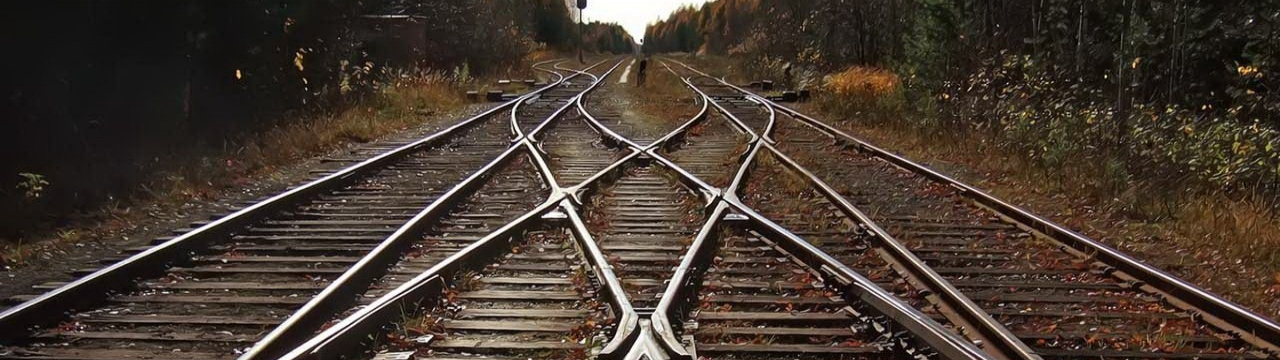
\includegraphics[scale=1.53]{../System/railway_track.jpg}
	\label{fig:track}
\end{figure}
	\vspace*{0.167\textheight}
	\textbf{\LARGE Docker Implementation}\\[\baselineskip]
    \textbf{\textcolor{MyBlue}{\Huge R\Large ailway \Huge A\Large dministration and \Huge I\Large nformation \Huge L\Large ogical \Huge S\Large ystem}}\\[\baselineskip]
	{\Large \textit{RAILS for Model Railroads}}
	\vfill
    \vspace*{\baselineskip}
	{\small David Bristow}

	{\small Version 1.0.0}
	
	{\small \today}
	\vspace*{3\baselineskip}
\end{titlepage}
%%========================================================================
\tableofcontents
%% copyright notice
%%========================================================================
\chapter{Microcontrollers for RAILS}
\section{Introduction}
\gls{rails} is a software model and implementation of an automated system to assist the model railroader achieve realism in the operation of a model railroad.
There are four user interface \gls{spa} that provide different aspects of rails they are:
\begin{itemize}
  \item \gls{rsrm} allows the user to match a rfid tag to a rollingstock's road name and number;
  \item \gls{mrim} allows the user to create, update and delete model railroad assets, such as rolling stock;
  \item \gls{mppm} allows the user to enter information about their projects and purchases; and
  \item \gls{mrlm} allows the user to enter information about their layout and control elements of it.
\end{itemize}
\section{RSRM Components}
The implementation of \gls{rsrm} consists of the following micro-services components:
\begin{itemize}
\item \gls{rfid} Controller is a micro-controller that processes \gls{rfid} tags obtained from a \gls{rfid} reader and then publishes \gls{iot} messages to the \gls{mqtt} Broker;
\item \gls{mqtt} Broker is responsible for receiving \gls{rfid} and micro info messages, filtering them, posting to designated topics and sending messages to clients subscribing to topics. The subscribers and publishers bridge the \gls{mqtt} elements with the GUI applications. The broker handles \gls{iot} messages;
\item \gls{isrs} subscribes to \gls{rfid} messages and pushes them via a web-socket to the rsm component;
\item \gls{isms} that subscribes to micro controller startup and heartbeat messages, updating the micros collection via \gls{rlds};
\item \gls{rlds} provides \gls{rest} access to model railroad layout collections including micros;
\item \gls{rids} provides \gls{rest} access to railroad inventory collections including rollingstock;
\item MongoDB a NoSQL database program that stores data records as documents which are gathered in collections. A database stores one or more collections of documents;
\item \gls{mr} Data is the document repository, used by MongoDB, to store complete collections of items such as rollingstock, industries (producers and consumers), track elements, turnouts, projects, purchases, etc. in support of \gls{rails}; and
\item \gls{rsrm} is the \gls{spa} that allows a user to match a \gls{rfid} tag to a rollingstock's road name and number.
\end{itemize}
Figure \ref{fig:rsms-ms-components} depicts the micro-services used to create the rolling stock \gls{rfid} management subsystem.

\begin{figure}[H]
	\centering
		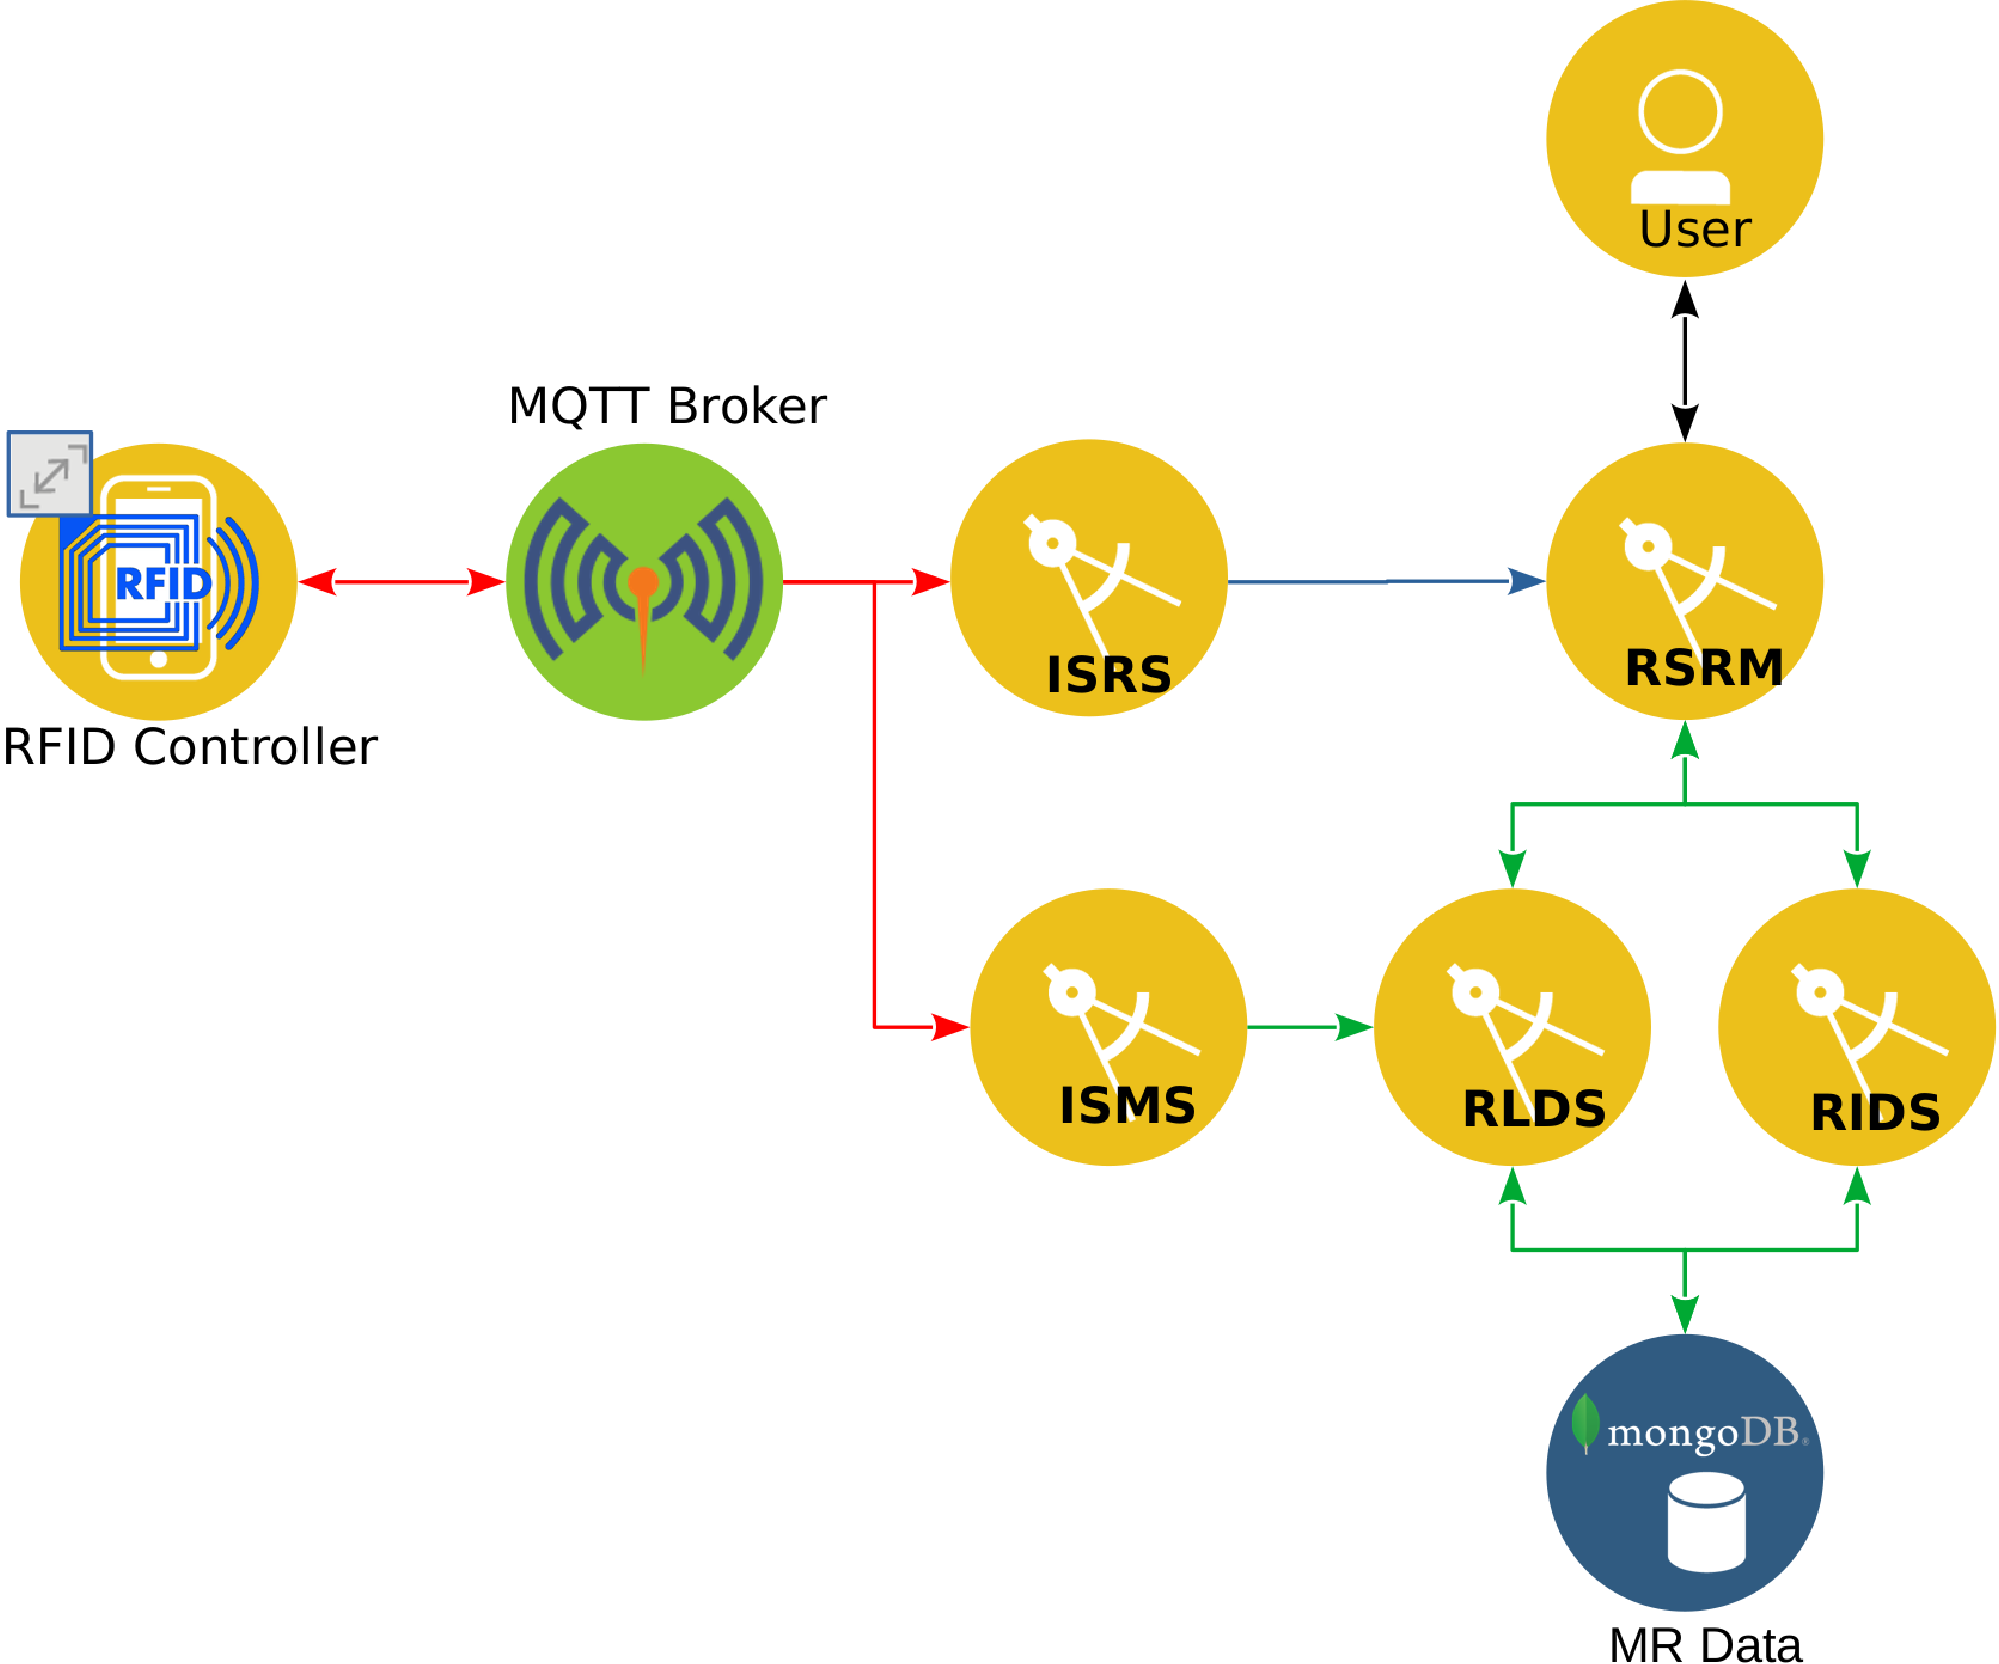
\includegraphics[scale=0.15]{../Images/rsms_microservices.png}
	\caption{Microservices Components}
	\label{fig:rsms-ms-components}
\end{figure}

Three system components that make up this subsystem:
\begin{itemize}
\item \gls{rfid} Controller is a micro-controller that processes \gls{rfid} tags obtained from a \gls{rfid} reader and then publishes \gls{iot} messages to the \gls{mqtt} Broker;
\item Network is a \gls{tcpip} communication medium that connects the \gls{rfid} Controller, \gls{mqtt} Broker and \gls{rsrm} components; and
\item Host is a computer that runs the \gls{mqtt} Broker and other \gls{rsrm} micro-services components.
\end{itemize}
Figure \ref{fig:rsms-system} depicts the systems components used to create the rolling stock \gls{rfid} management subsystem.

\begin{figure}[H]
	\centering
		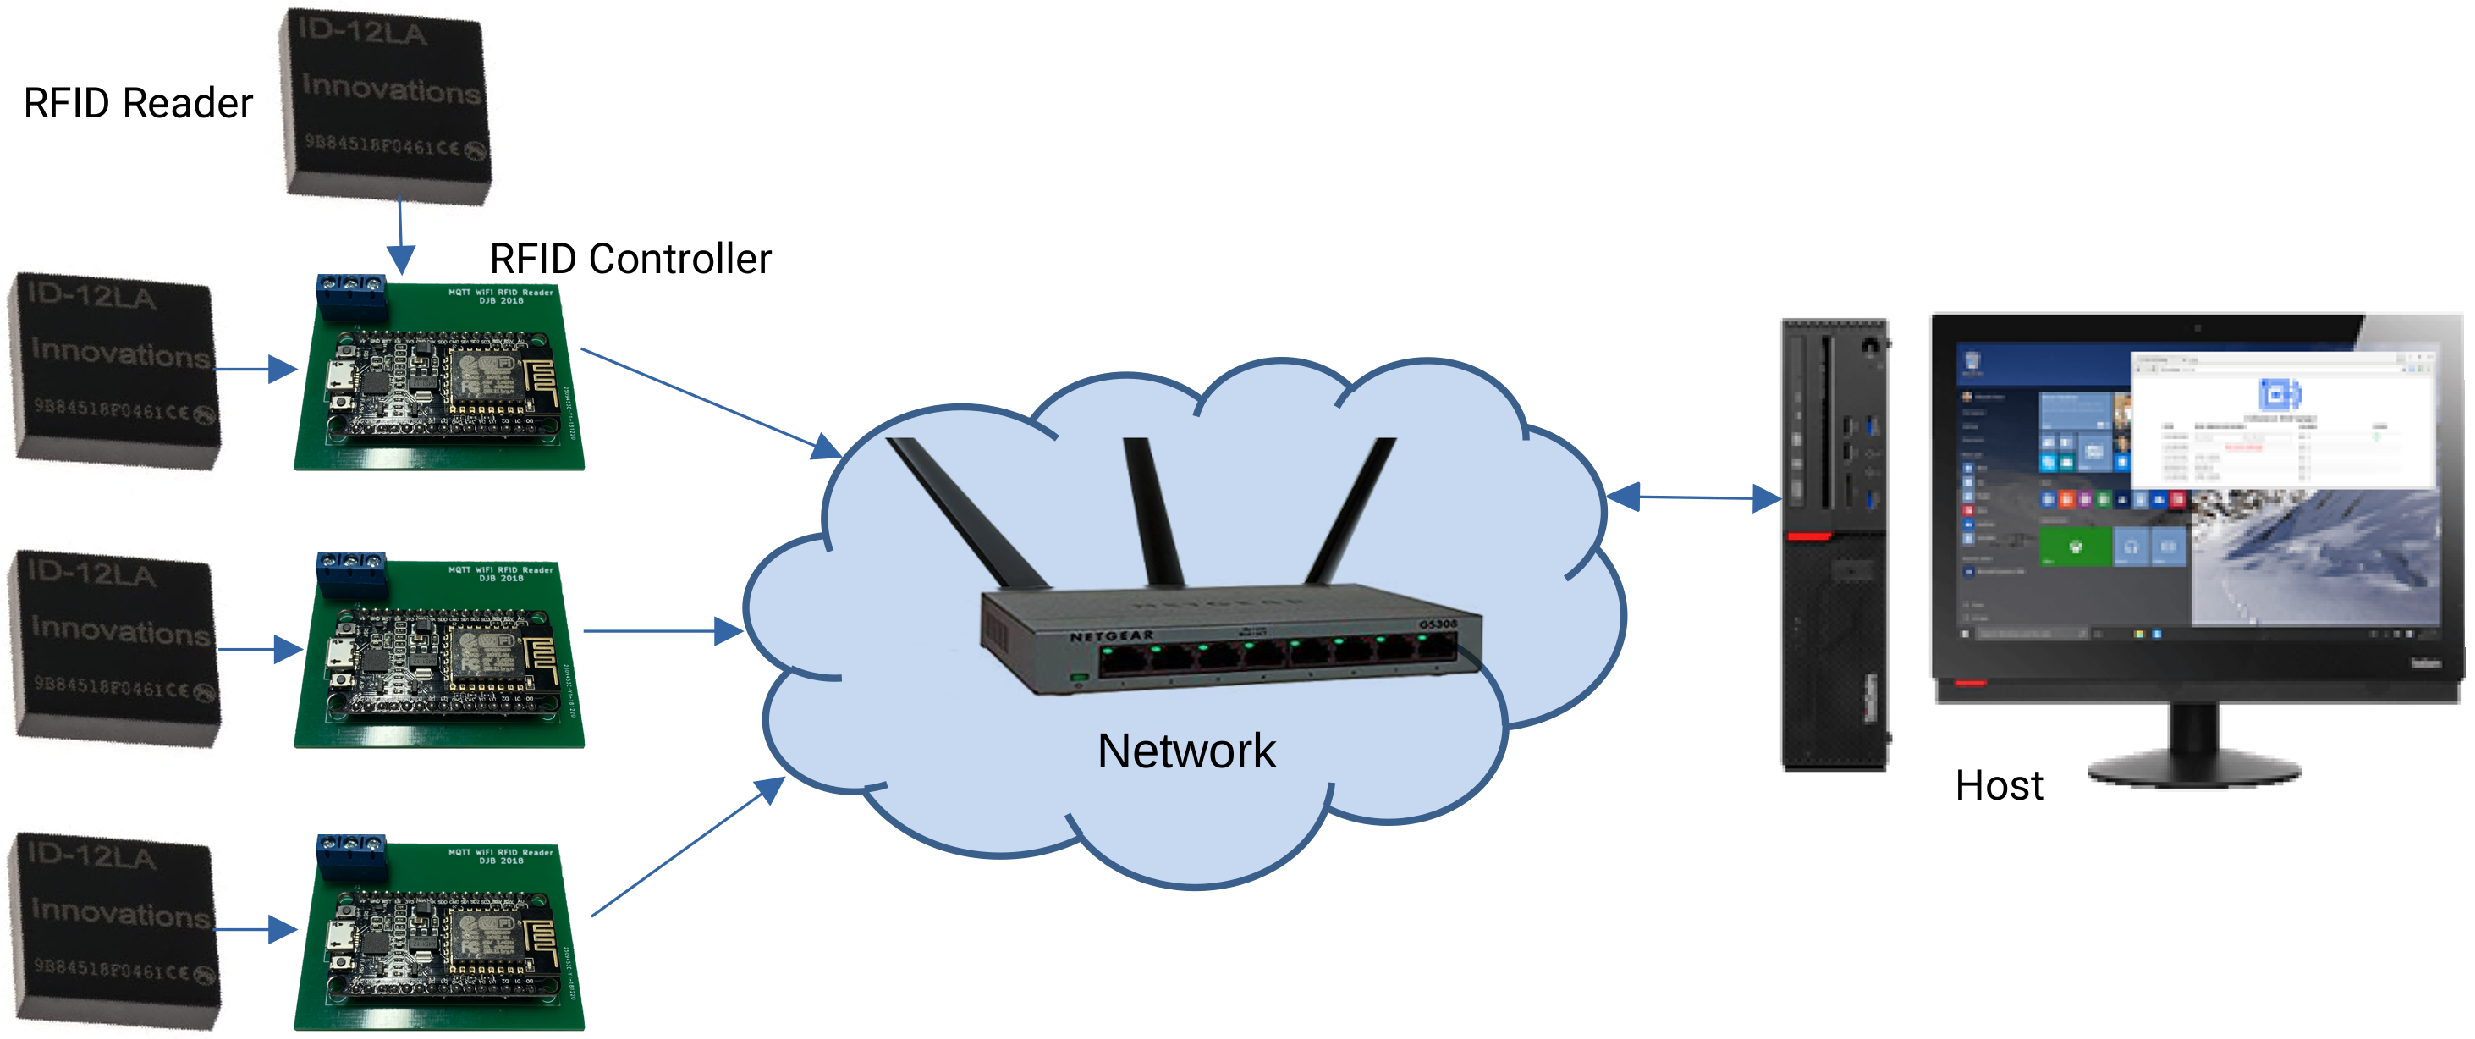
\includegraphics[scale=0.15]{../Images/rsms_system.png}
	\caption{RSMS System Components}
	\label{fig:rsms-system}
\end{figure}

\section{MRLM System Components}

Figure \ref{fig:mrlm-ms-components} depicts the micro-services used to create the \gls{mrlm} subsystem and figure \ref{fig:turnout-system} depicts it's logical architecture.

\begin{figure}[H]
	\centering
		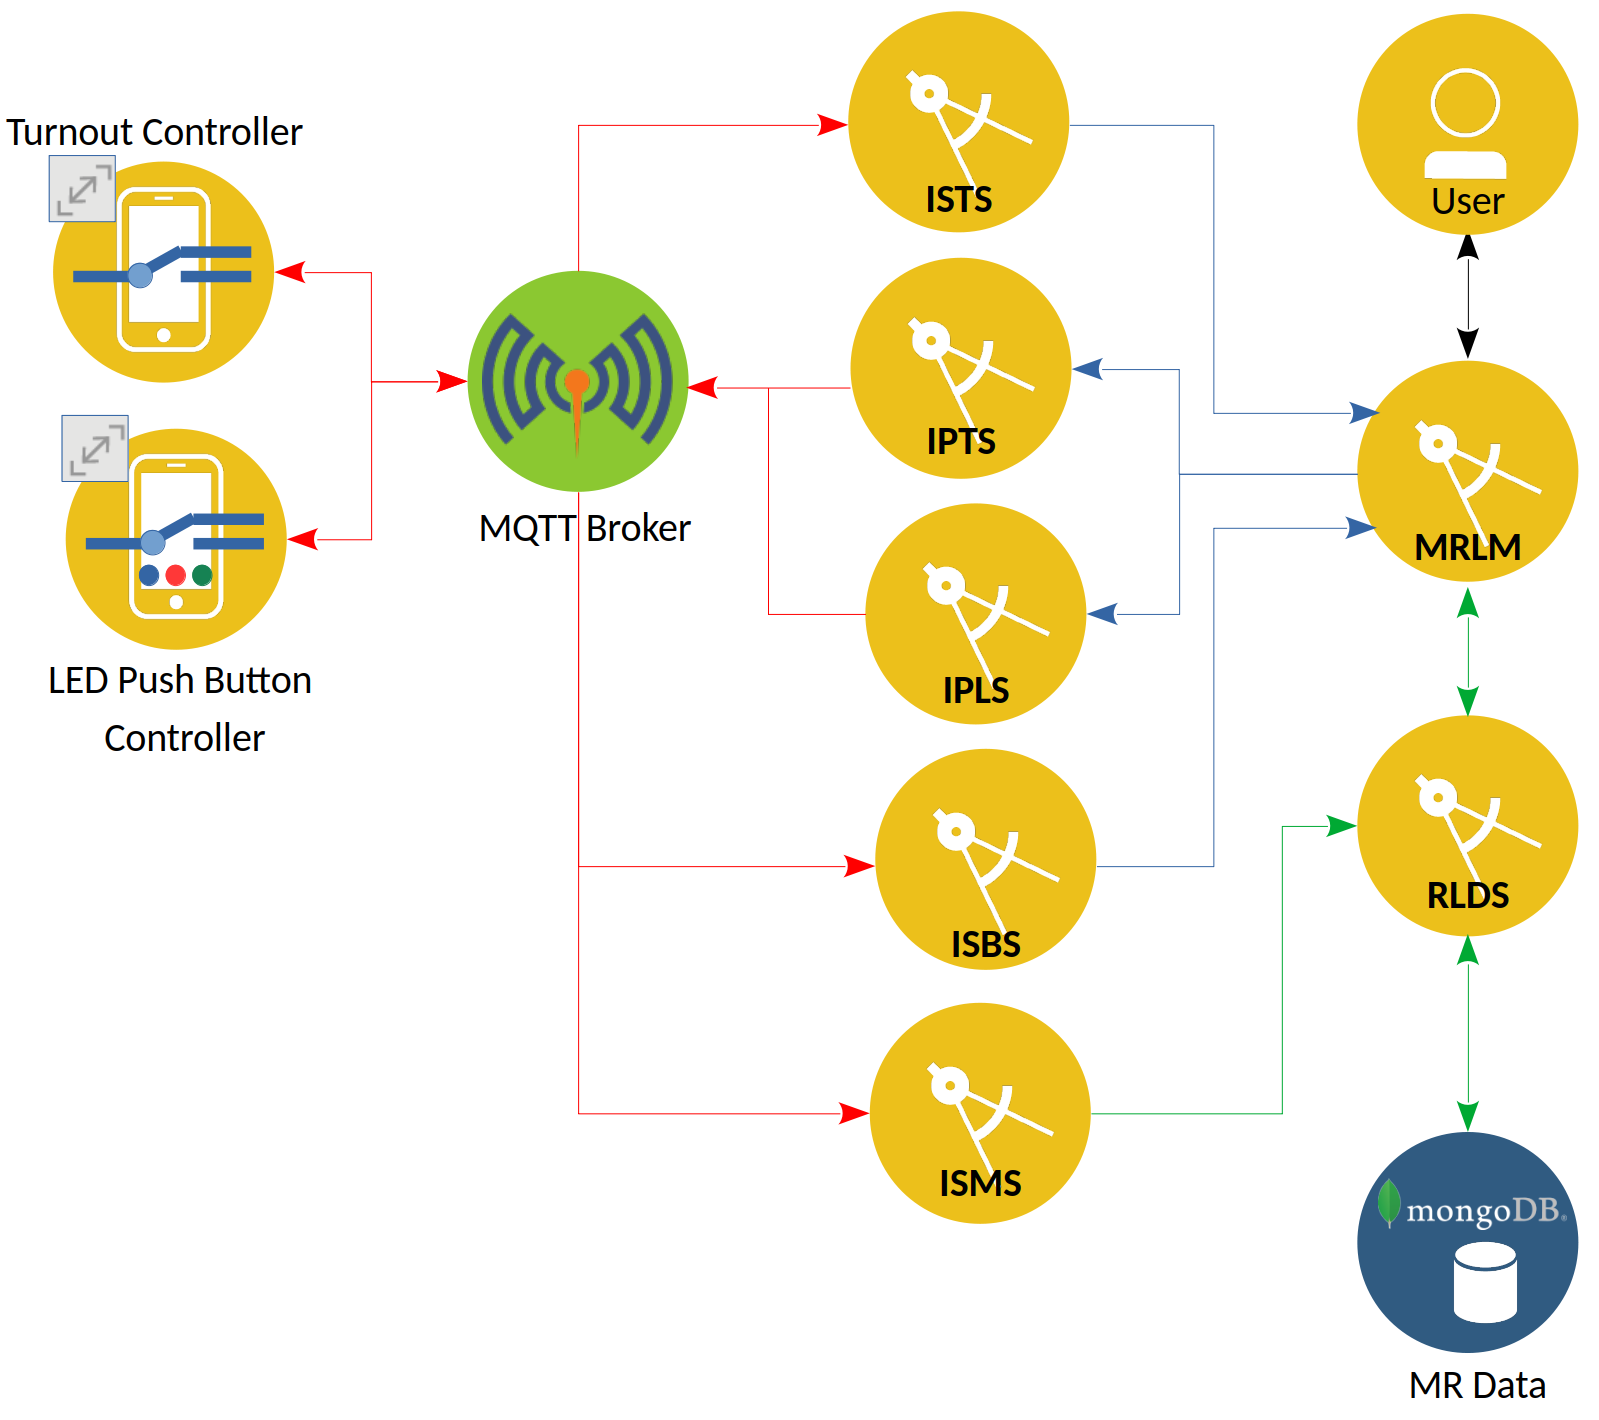
\includegraphics[scale=0.2]{../Images/mrlm_microservices.png}
	\caption{Microservices Components}
	\label{fig:mrlm-ms-components}
\end{figure}


\begin{figure}[H]
	\centering
		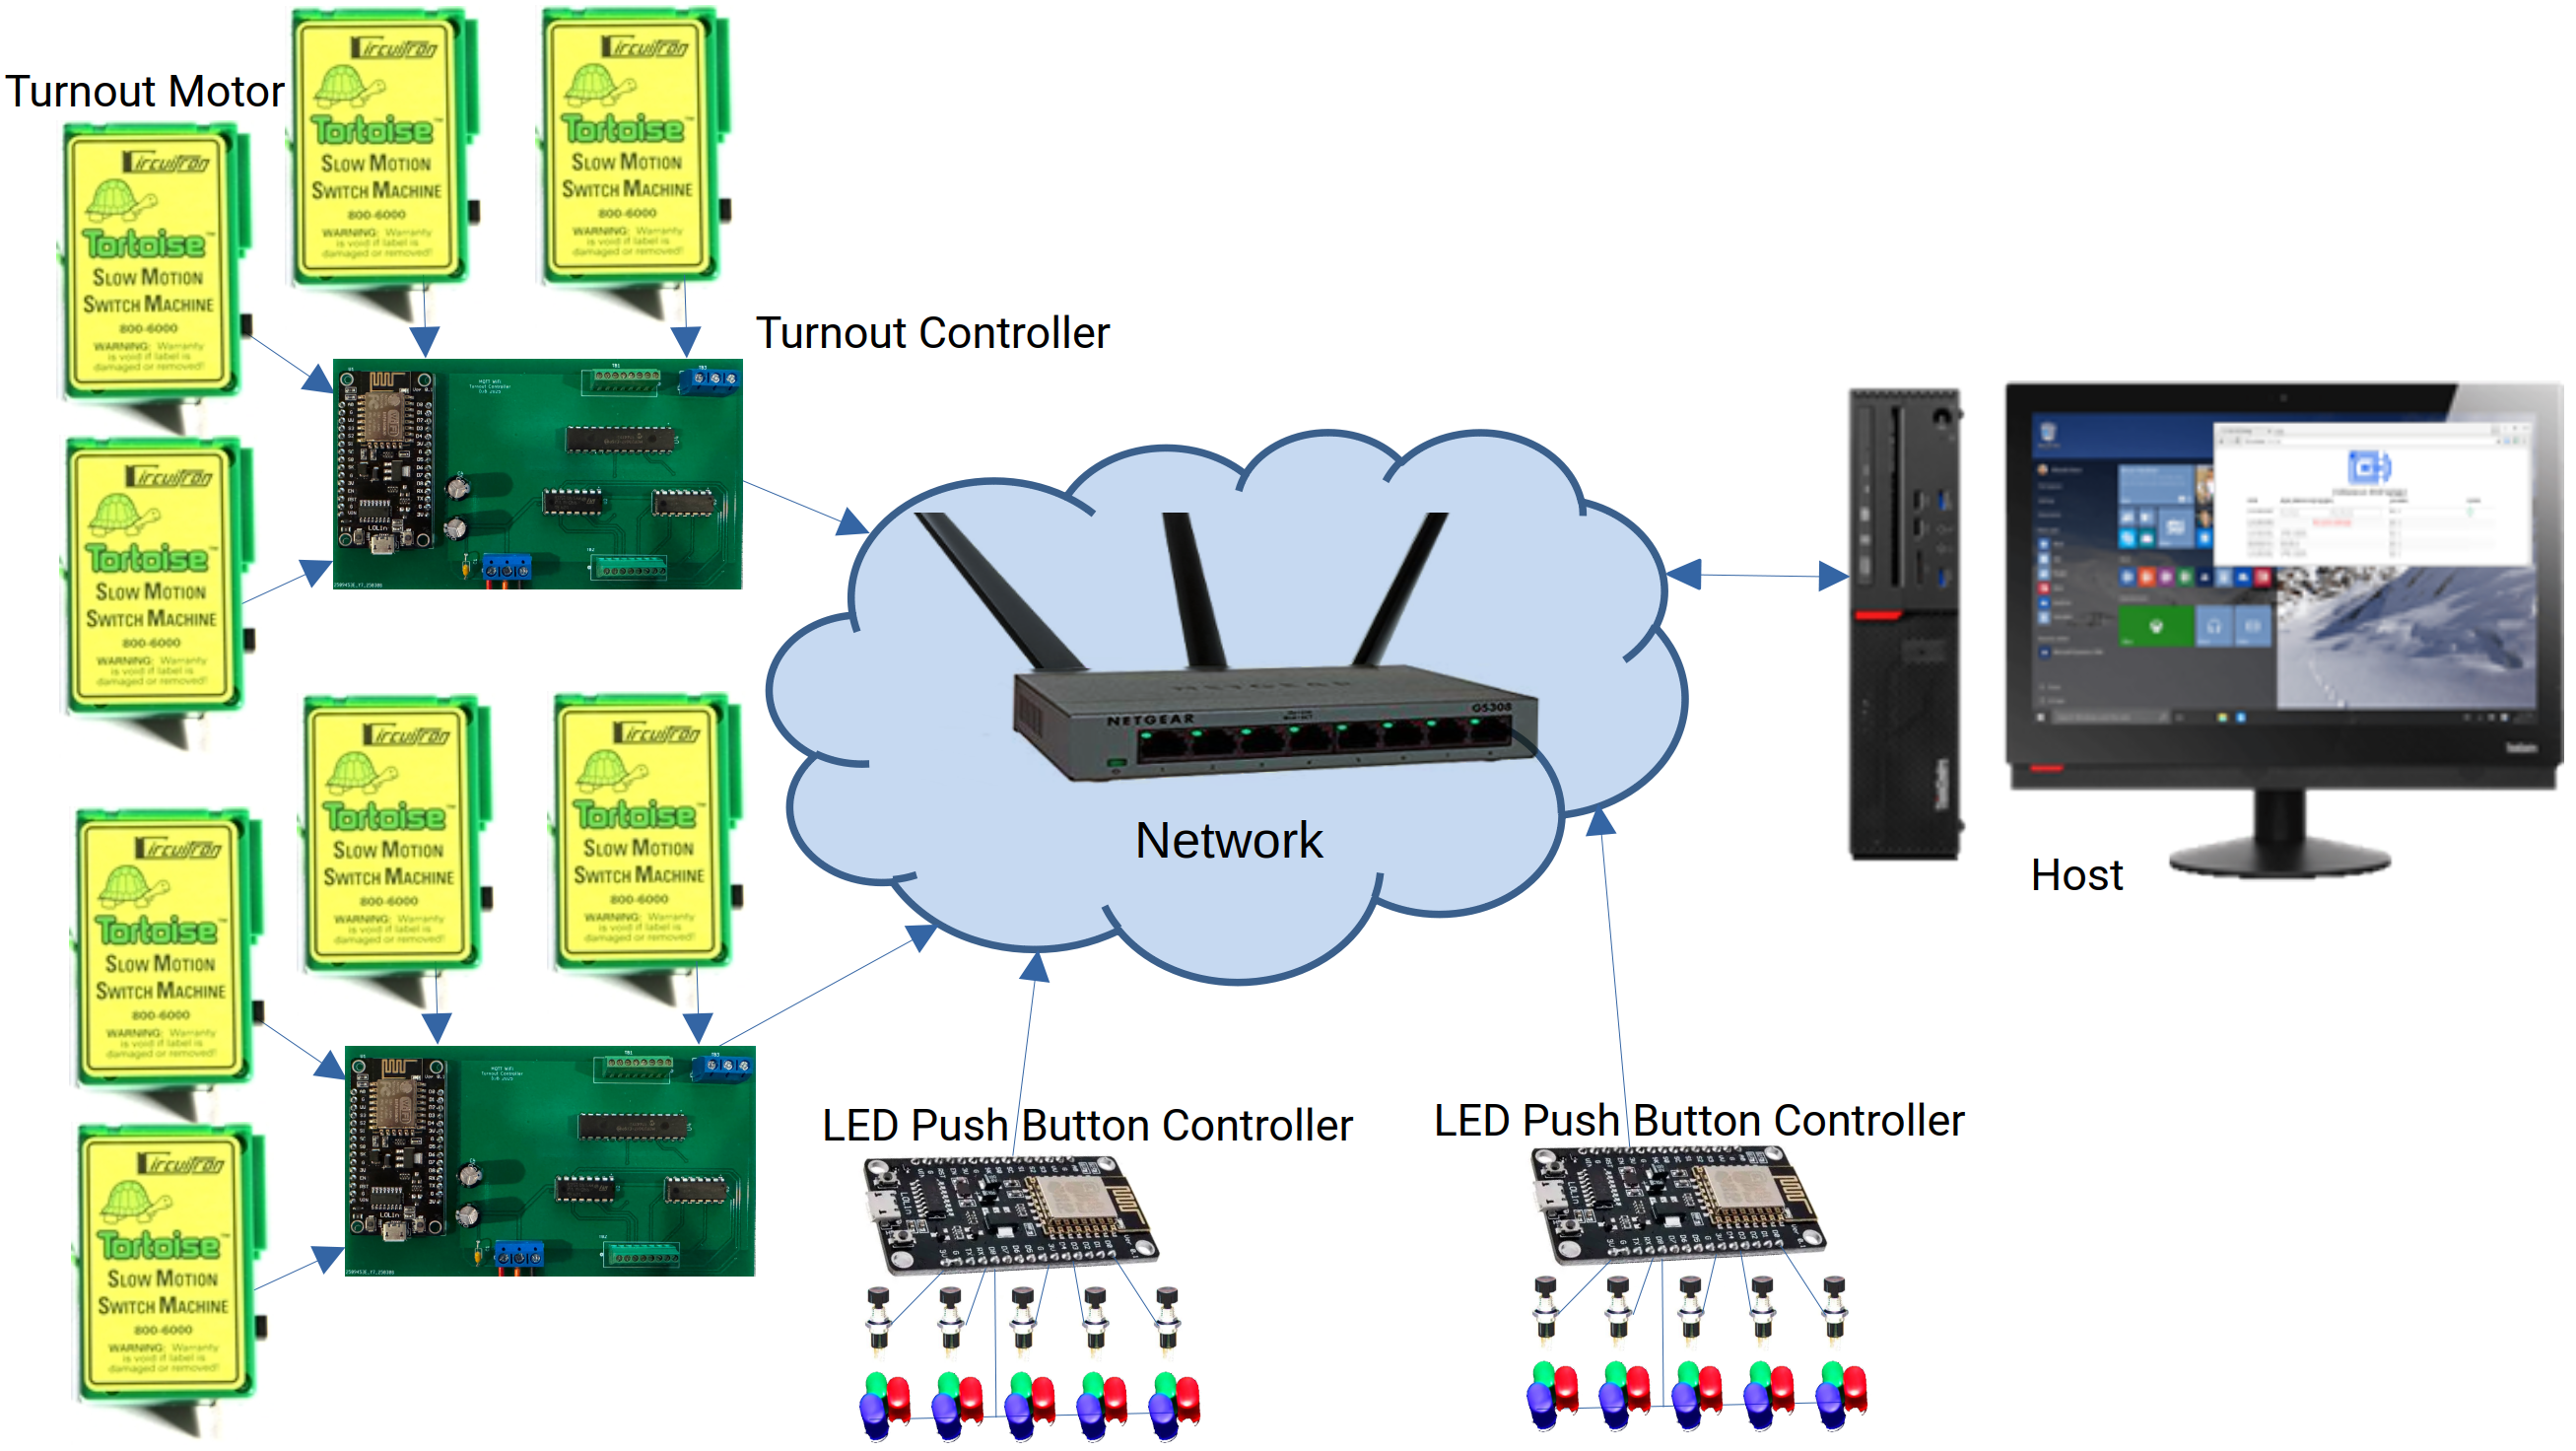
\includegraphics[scale=0.2]{../Images/mrlm_system.png}
	\caption{MRLM System Components}
	\label{fig:turnout-system}
\end{figure}

\chapter{Setup and Run}
\label{ch:installandrun}
\section{Docker Installation}
\label{sec:dockerinstall}
The \gls{rails} \glspl{spa} are implemented as Docker containers. The Docker containers are built and pushed to Docker Hub. The Docker containers are then pulled from Docker Hub and run on the host machine. 
The host machine must have Docker installed. Docker is a platform for developing, shipping, and running applications in containers. Docker can be installed on Windows, macOS, and Linux. 
The installation instructions for Docker can be found at \href{https://docs.docker.com/get-docker/}{https://docs.docker.com/get-docker/}.
\section{Docker Compose Installation}
\label{sec:dockercomposeinstall}
Docker Compose is a tool for defining and running multi-container Docker applications. Docker Compose uses a YAML file to configure the application's services. The installation instructions\footnote{Note that for Microsoft Windows the installation of the \gls{gui} Docker Desktop automatically installs Docker Compose.} for Docker Compose can be found at \href{https://docs.docker.com/compose/install/}{https://docs.docker.com/compose/install/}.  The Docker Compose file for the \gls{rails} \glspl{spa} is shown in Appendix \ref{app:yamlfile}.
\section{Broker Configuration}
\label{sec:brokerconfig}
The \gls{rails} \glspl{spa} use the Mosquitto broker to communicate with each other. The Mosquitto broker is an open-source message broker that implements the \gls{mqtt} protocol. The Mosquitto broker must be configured to allow the \gls{rails} \glspl{spa} to communicate with each other. The Mosquitto broker configuration file must be edited to allow the \gls{rails} \glspl{spa} to communicate with each other. The configuration file is found in the virtual storage whose volume name is “mosquitto”. To establish and modify the configuration file the following steps are taken:
\begin{enumerate}
    \item Create a Docker volume for the Mosquitto broker.
    \begin{verbatim}
    docker volume create --name mosquitto
    \end{verbatim}
    \item Run a Docker container for the first time the Mosquitto broker, which will create the initial configuration file.
    \begin{verbatim}
    docker run -it --name myMqttBrkr -p 1883:1883 -p 9001:9001 --rm
    -v mosquitto:/mosquitto -d eclipse-mosquitto
    \end{verbatim}
    \item Stop the broker container.
    \begin{verbatim}    
    docker stop myMqttBrkr
    \end{verbatim}
    \item Locate the configuration file in the "mosquitto" volume.
    \begin{verbatim}    
    docker inspect mosquitto
    \end{verbatim}
    \item Edit the configuration file modifying or adding the following lines:
    \begin{verbatim}
    listener 1883
    allow_anonymous true
    socket_domain ipv4
    \end{verbatim}
\end{enumerate}
\section{Create the RAILS Docker Environment}
\label{sec:railsdockerenv}
The \gls{rails} \glspl{spa} are implemented as Docker containers that require an environment to run in. To create that environment, the following steps are taken:
\begin{enumerate}
    \item Create a Docker volume for the Rails database.
    \begin{verbatim}
    docker volume create --name myRailsDb  
    \end{verbatim}
    \item Create a Docker volume for the Rails images.
    \begin{verbatim}
    docker volume create --name myRailsImages
    \end{verbatim}
    \item Create a Docker network for the Rails containers to communicate over.
    \begin{verbatim}
    docker network create myRailsNet
    \end{verbatim}
\end{enumerate}
\section{Run the RAILS Docker Containers}
\label{sec:railsdockercontainers}
The Docker containers are pulled from Docker Hub and run on the host machine. To run all of the \gls{rails} Docker containers, either create the YAML file from Appendix \ref{app:yamlfile} or retrieve the YAML file from the \gls{rails} GitHub repository found at \href{https://github.com/djbristow/RAILS/tree/master/Docker%20Based}{my GitHub repository}. The YAML file is used to run the \gls{rails} Docker containers.  
to run all four \gls{rails} Docker containers, the following command in the directory where the YAML file is located:
\begin{verbatim}
docker-compose up -d
\end{verbatim}
If the \gls{rails} Docker \gls{spa} containers are to be run individually, the following commands are used:
\begin{verbatim}
docker-compose up -d myMrim
docker-compose up -d myRsrm
docker-compose up -d myMppm
docker-compose up -d myMrlm
\end{verbatim}
Point a browser, on the host machine, to the following URLs to access the \gls{rails} \glspl{spa}:
\begin{itemize}
    \item \gls{mrim} \gls{spa} - \href{http://localhost/mrim}{http://localhost/mrim} (or \texttt{http://\textless MACHINE\_IP\textgreater /mrim/})
    \item \gls{rsrm} \gls{spa} - \href{http://localhost/rsrm}{http://localhost/rsrm} (or \texttt{http://\textless MACHINE\_IP\textgreater /rsrm/})
    \item \gls{mppm} \gls{spa} - \href{http://localhost/mppm}{http://localhost/mppm} (or \texttt{http://\textless MACHINE\_IP\textgreater /mppm/})
    \item \gls{mrlm} \gls{spa} - \href{http://localhost/mrlm}{http://localhost/mrlm} (or \texttt{http://\textless MACHINE\_IP\textgreater /mrlm/})
\end{itemize}
Where \textless MACHINE\_IP\textgreater is the IP address of the host machine running the Docker containers. The \gls{rails} \glspl{spa} can be accessed from any browser on any Personal Computer (PC) in the network.
\section{Stop and Remove the RAILS Docker Containers}
\label{sec:stopremoverailsdockercontainers}
To stop and remove the \gls{rails} Docker containers, the following command is used:
\begin{verbatim}
docker-compose down
\end{verbatim}

See Appendix \ref{app:examplecommands} for screenshots of the Docker commands used to create the Docker environment and run the \gls{rails} \glspl{spa}.
\chapter{Alternate Approach} 
\label{ch:altsapproach}
An alternate approach to setting up and running the set of \glspl{spa} to implement \gls{rails} is to use Docker containers directly. Docker must have been installed on the host machine. The Docker images for the \gls{rails} \glspl{spa} must have been built and pushed to Docker Hub. It is anticipated that the reader has a basic understanding of Docker and how to use it.\\
To create the Docker envirnment for the \gls{rails} \glspl{spa} to run in, the following steps are taken:
\begin{enumerate}
    \item Create a Docker volume for the Mosquitto broker. Refer to section \ref{sec:brokerconfig} for information on configuring the Mosquitto broker.
    \begin{verbatim}
    docker volume create --name mosquitto
    \end{verbatim}
    \item Create a Docker volume for the Rails database.
    \begin{verbatim}
    docker volume create --name myRailsDb  
    \end{verbatim}
    \item Create a Docker volume for the Rails images.
    \begin{verbatim}
    docker volume create --name myRailsImages
    \end{verbatim}
    \item Create a Docker network for the Rails conatiners to communicate over.
    \begin{verbatim}
    docker network create myRailsNet
    \end{verbatim}
    \item Run a Docker container for the MongoDB database.
    \begin{verbatim}
    docker run --network myRailsNet --name myMongo -v myRailsDb:/data/db
    -p 27017:27017 -d mongo
    \end{verbatim}
    \item Run a Docker container for the \gls{ppds} \gls{ds}.
    \begin{verbatim}
    docker run --network myRailsNet --name myPpds -p 3007:3007 -d dbristow/ppds
    \end{verbatim}
    \item Run a Docker container for the \gls{rids} \gls{ds}.
    \begin{verbatim}
    docker run --network myRailsNet --name myRids -p 3000:3000 -d dbristow/rids
    \end{verbatim}
    \item Run a Docker container for the \gls{rlds} \gls{ds}.
    \begin{verbatim}
    docker run --network myRailsNet --name myRlds -p 3006:3006 -d dbristow/rlds
    \end{verbatim}
    \item Run a Docker container for the \gls{mrfm} \gls{ds}.
    \begin{verbatim}
    docker run --network myRailsNet --name myMrfm -v myRailsImages:/usr/djb/src/uploads 
    -p 3030:3030 -d dbristow/mrfm
    \end{verbatim}
    \item Run a Docker container for the Mosquitto broker.
    \begin{verbatim}
    docker run --network myRailsNet -it --name myMqttBrkr -p 1883:1883 -p 9001:9001
    -v mosquitto:/mosquitto -d eclipse-mosquitto
    \end{verbatim}
    \item Run a Docker conatainer for the \gls{isrs} \gls{iots}.
    \begin{verbatim}
    docker run --network myRailsNet -p 3005:3005 --name myIsrs -d dbristow/isrs
    \end{verbatim}
    \item Run a Docker conatainer for the \gls{isms} \gls{iots}.
    \begin{verbatim}
    docker run --network myRailsNet --name myIsms -d dbristow/isms
    \end{verbatim}
    \item Run a Docker conatainer for the \gls{ists} \gls{iots}.
    \begin{verbatim}
    docker run --network myRailsNet -p 3010:3010 --name myIsts -d dbristow/ists
    \end{verbatim}
    \item Run a Docker conatainer for the \gls{isbs} \gls{iots}.
    \begin{verbatim}
    docker run --network myRailsNet -p 3012:3012 --name myIsbs -d dbristow/isbs
    \end{verbatim}
    \item Run a Docker conatainer for the \gls{ipts} \gls{iots}.
    \begin{verbatim}
    docker run --network myRailsNet -p 3011:3011 --name myIpts -d dbristow/ipts
    \end{verbatim}
    \item Run a Docker conatainer for the \gls{ipls} \gls{iots}.
    \begin{verbatim}
    docker run --network myRailsNet -p 3013:3013 --name myIpls -d dbristow/ipls
    \end{verbatim}
    \item Run a Docker container for the \gls{rsrm} \gls{spa}.
    \begin{verbatim}
    docker run --network myRailsNet -p 3002:8080 --name myRsrm -d dbristow/rsrm
    \end{verbatim}
    \item Run a Docker container for the \gls{mppm} \gls{spa}.
    \begin{verbatim}
    docker run --network myRailsNet -p 3008:8080 --name myMppm -d dbristow/mppm
    \end{verbatim}
    \item Run a Docker container for the \gls{mrim} \gls{spa}.
    \begin{verbatim}
    docker run --network myRailsNet -p 3001:8080 --name myMrim -d dbristow/mrim
    \end{verbatim}
    \item Run a Docker container for the \gls{mrlm} \gls{spa}.
    \begin{verbatim}
    docker run --network myRailsNet -p 3004:8080 --name myMrlm -d dbristow/mrlm
    \end{verbatim}
\end{enumerate}
This approach is more complex than the Docker Compose approach, but it allows for more control over the individual containers. Completing all the steps above will result in running the four \gls{rails} \glspl{spa}.\vspace{5mm}\\
Once the containers are running, the \glspl{spa} can be accessed by pointing a web browser to the appropriate URL. The \gls{mrim} \gls{spa} is accessed at http://localhost:3001, the \gls{rsrm} \gls{spa} is accessed at http://localhost:3002, the \gls{mppm} \gls{spa} is accessed at http://localhost:3008, and the \gls{mrlm} \gls{spa} is accessed at http://localhost:3004.\vspace{5mm}\\  
If only the \gls{mrim} \gls{spa} is desired, the following steps should be taken in order: 2, 3, 4, 5, 7, 9, and 19\\
If only the \gls{rsrm} \gls{spa} is desired, the following steps should be taken in order: 1, 2, 4, 5, 7, 8, 10, 11, 12 and 17\\
If only the \gls{mppm} \gls{spa} is desired, the following steps should be taken in order: 2, 4, 6, and 18\\
If only the \gls{mrlm} \gls{spa} is desired, the following steps should be taken in order: 2, 4, 5, 8, 10, 12, 13, 14,15, 16, and 20\\

\appendix
\chapter{YAML File}
\label{app:yamlfile}

\lstdefinelanguage{YAML}{
    morekeywords={image, container_name, networks, ports, volumes, depends_on, services, version, external, volumes},
    keywordstyle=\color{bluekeywords},
    sensitive=false,
    morecomment=[l][\color{greencomments}]{\#},
    morecomment=[l][\color{greencomments}]{//},
    morecomment=[s][\color{greencomments}]{{(*}{*)}},
    morestring=[b]",
    morestring=[b]',
    stringstyle=\color{redstrings}
    }

\lstset{
    backgroundcolor=\color{lightgray},
    basicstyle=\ttfamily\small,
    breaklines=true,
    frame=single,
    rulecolor=\color{black},
    language=YAML,
    captionpos=b,
    numbers=left,
    numberstyle=\tiny,
    }

\lstinputlisting[caption={docker compose file},label={lst:yaml}]{docker-compose.yaml}


\chapter{Example Setup and Run Commands}
\label{app:examplecommands}
The following screenshots show the Docker commands used to create the Docker environment and run the \gls{rails} Docker containers.
\section{Docker in a Windows Environment}
\label{sec:win-cmds}
Docker on Windows 11 relies on a component called \gls{wsl 2} to provide a Linux-like environment for running Docker containers. Docker Desktop installer provides two options:
\begin{itemize}
    \item Use \gls{wsl 2} backend: This is the recommended approach for most users. It leverages \gls{wsl 2} to create a Linux environment for Docker to run containers.
    \item Use Hyper-V backend: This is an alternative that uses Hyper-V virtualization technology. However, \gls{wsl 2} is generally considered more performant and resource-efficient.   
\end{itemize}
This setup is based on using WSL as it:
\begin{itemize}
    \item offers better performance for running Linux containers compared to Hyper-V.
    \item provides a more native Linux experience for Docker, ensuring compatibility with most Linux container images.
    \item uses the Windows kernel directly, leading to more efficient resource usage.
\end{itemize}
During Docker Desktop installation with the \gls{wsl 2} backend, Docker will automatically configure and set up \gls{wsl 2} if it's not already installed. It will also create a default Linux distribution (usually Ubuntu) within \gls{wsl 2}. Once \gls{wsl 2} is set up, Docker Desktop installs the Docker daemon within the \gls{wsl 2} environment. This daemon is the core process that manages Docker containers.
Docker Desktop provides a Docker \gls{cli} for Windows. This \gls{cli} interacts with the Docker daemon running in the \gls{wsl 2} environment through a remote API. So, when you run Docker commands on Windows, they are translated and sent to the Docker daemon in \gls{wsl 2} for execution.\vspace{5mm} \\
In essence, Docker on Windows 11 leverages \gls{wsl 2} to create a Linux-like environment for running Docker containers. This approach provides a powerful and performant solution for containerization on Windows, while still offering a familiar Windows experience for interacting with Docker.
\begin{figure}[H]
    \centering
    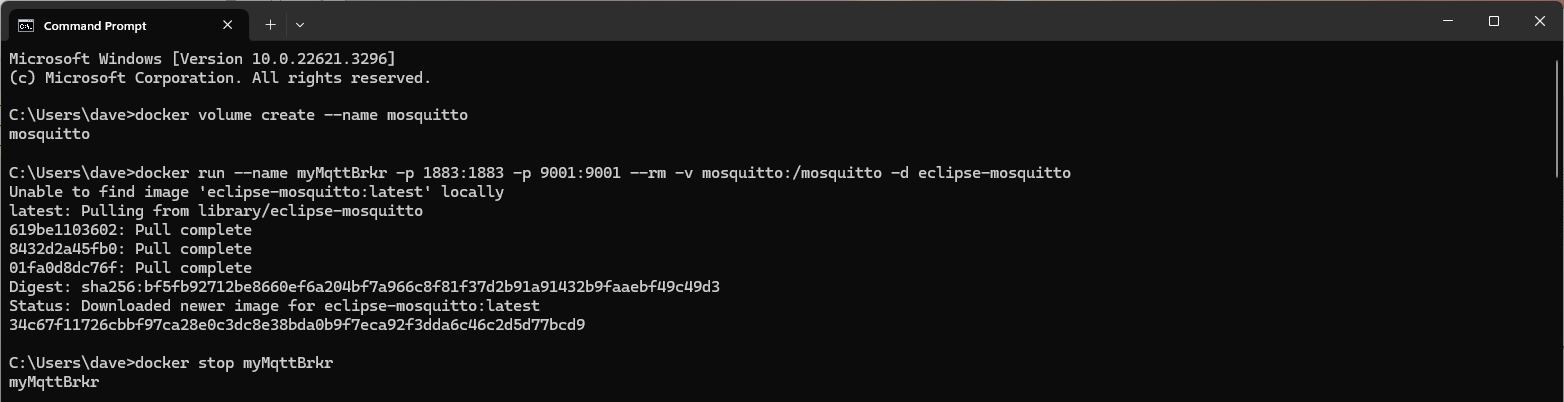
\includegraphics[scale=0.4]{win1.png}
    \caption{Intial Windows Docker Commands}
    \label{fig:init-docker-cmds}
\end{figure}
Docker Desktop with \gls{wsl 2} backend stores Docker images and volumes on the Windows file system, accessible from both Windows and \gls{wsl 2}. This allows for easy sharing of container data between the two environments. However, it simpler to use Docker Desktop \gls{gui} to locate and edit the mosquitto configuration file. The following screenshots show the location of he configuration file and the editing of the file.
\begin{figure}[H]
    \centering
    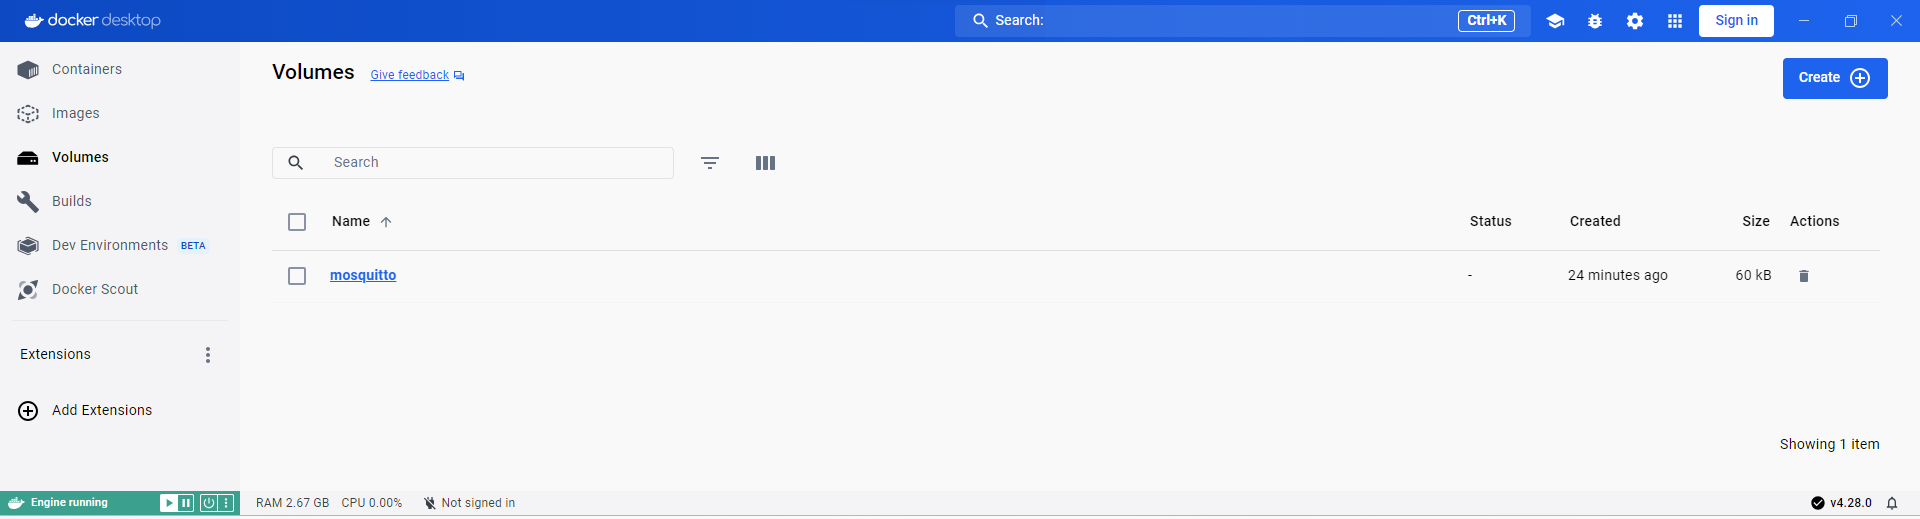
\includegraphics[scale=0.33]{volumes.png}
    \caption{Docker Desktop Volumes}
    \label{fig:mosquitto-volume}
\end{figure}
\begin{figure}[H]
    \centering
    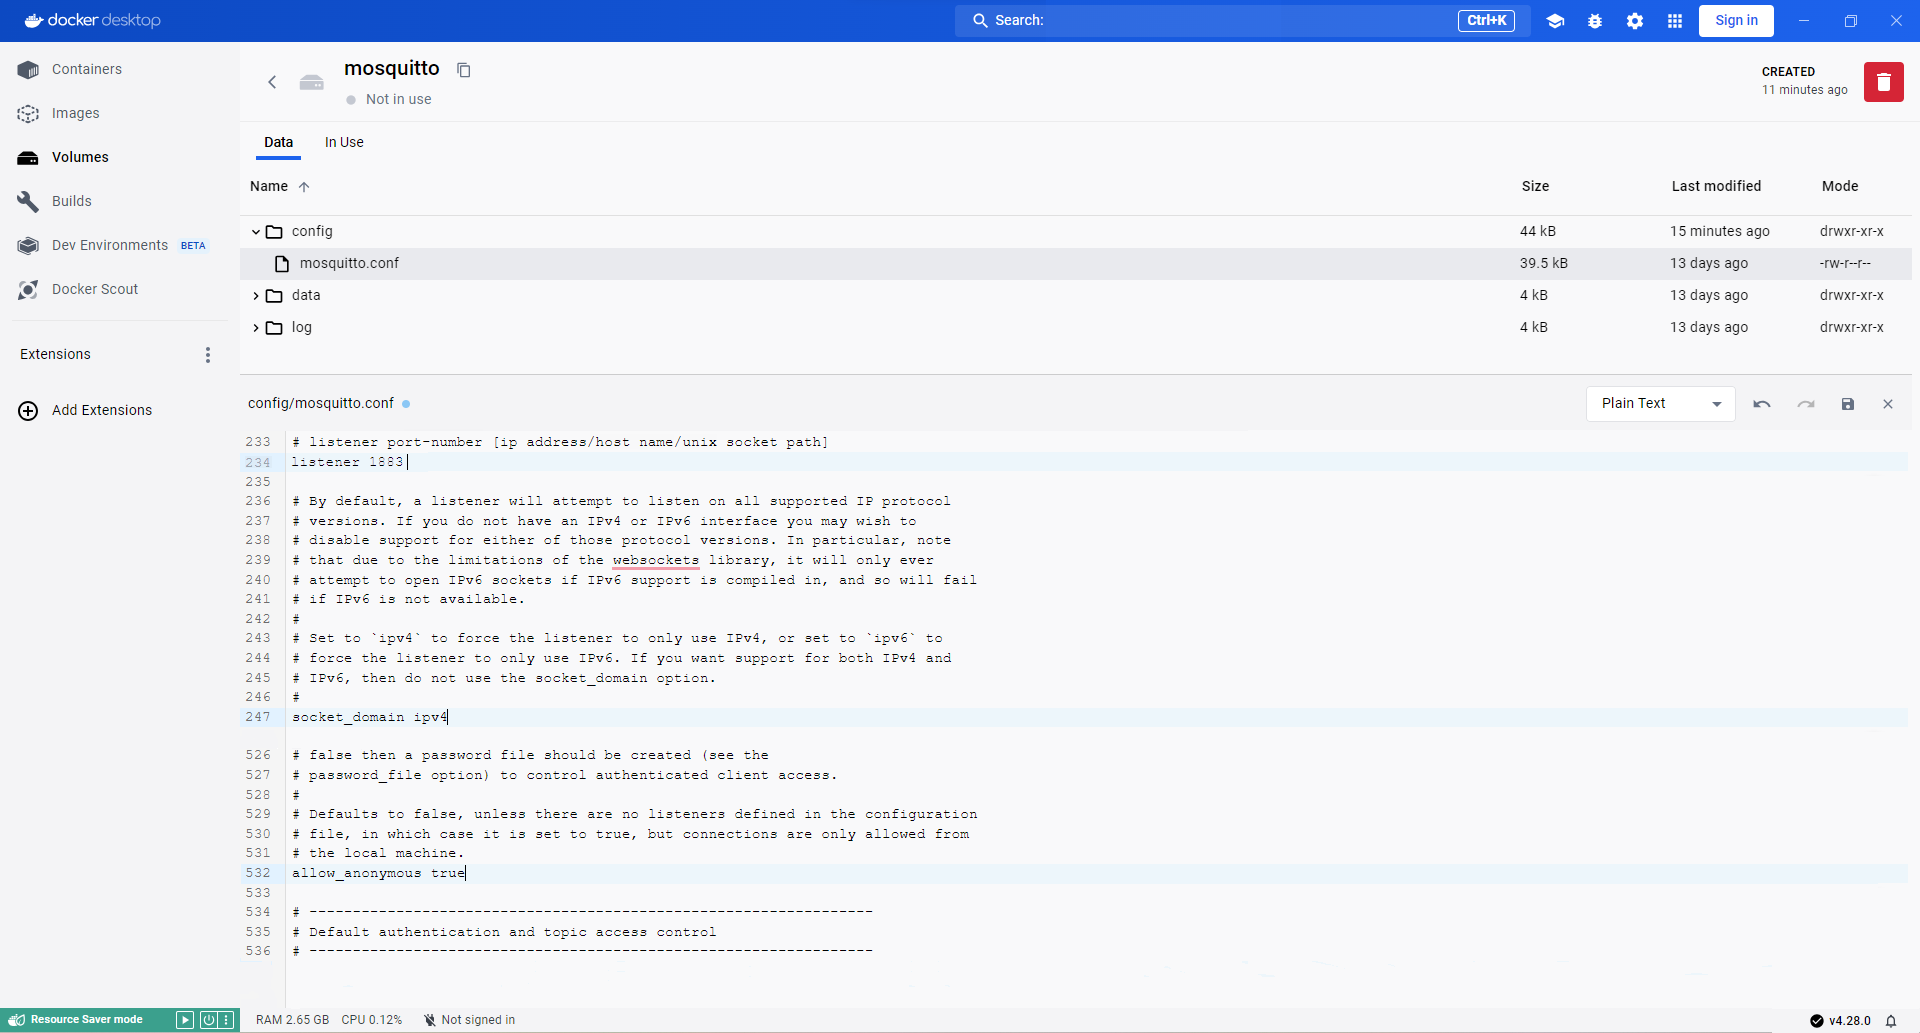
\includegraphics[scale=0.33]{edit-config.png}
    \caption{Mosquitto Configuration File}
    \label{fig:mosquitto-config}
\end{figure}
The following screenshots show the Docker commands used to create the Docker environment and run all of the \gls{rails} Docker containers.
\begin{figure}[H]
    \centering
    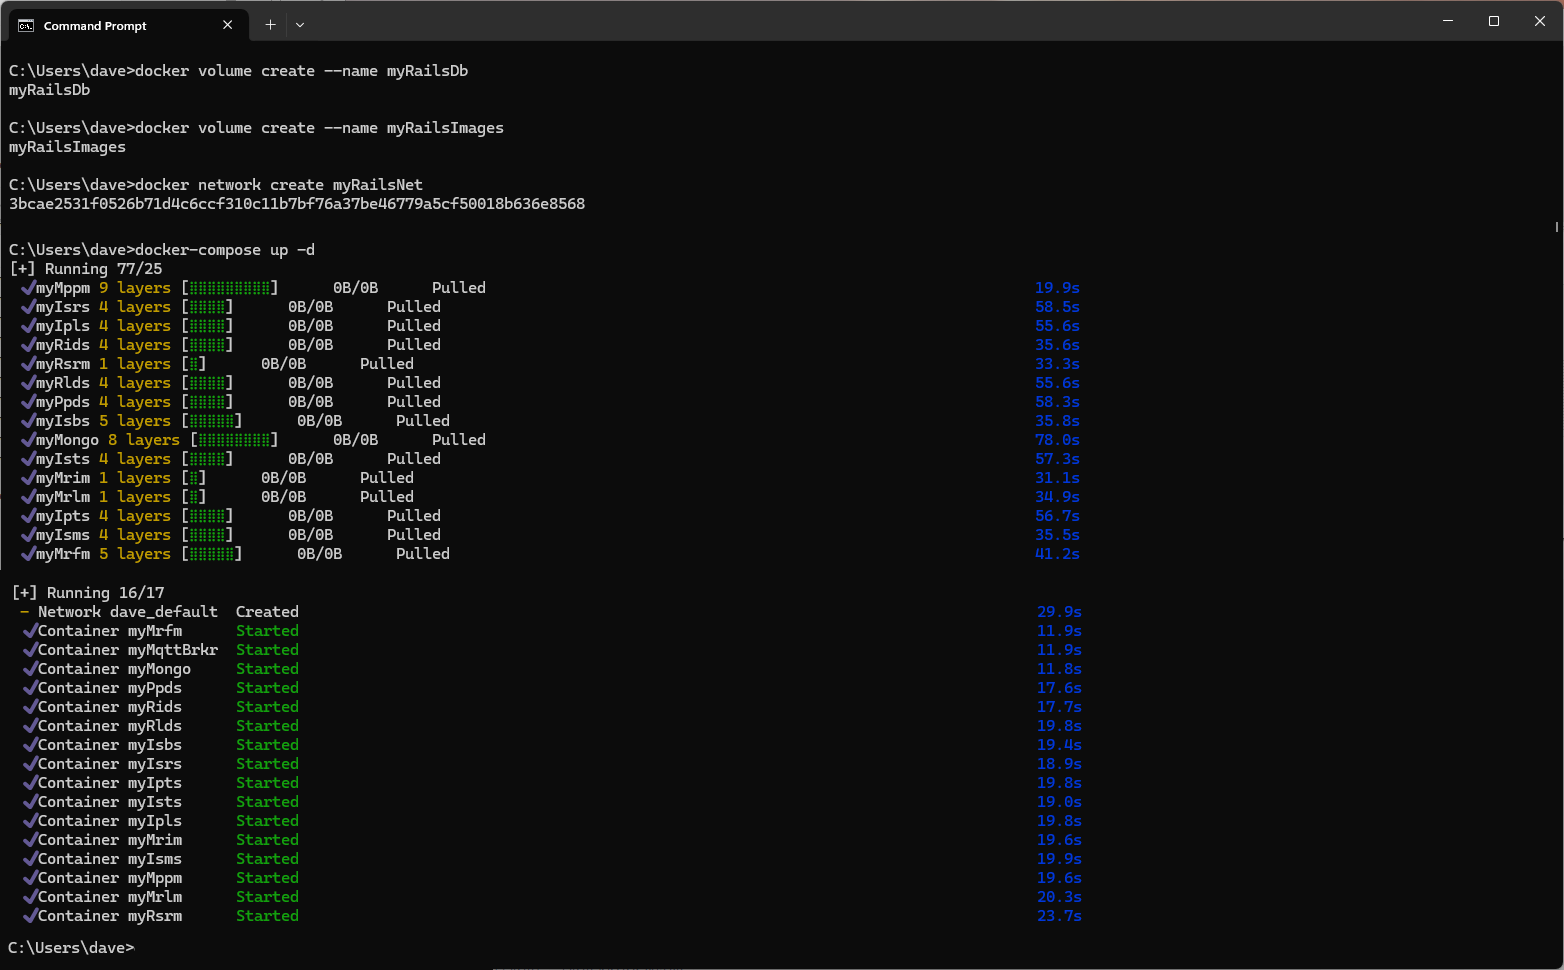
\includegraphics[scale=0.4]{win2.png}
    \caption{Windows Docker Commands Continued}
    \label{fig:docker-cmds} 
\end{figure}
The following screenshots confirm the Docker containers are running.
\begin{figure}[H]
    \centering
    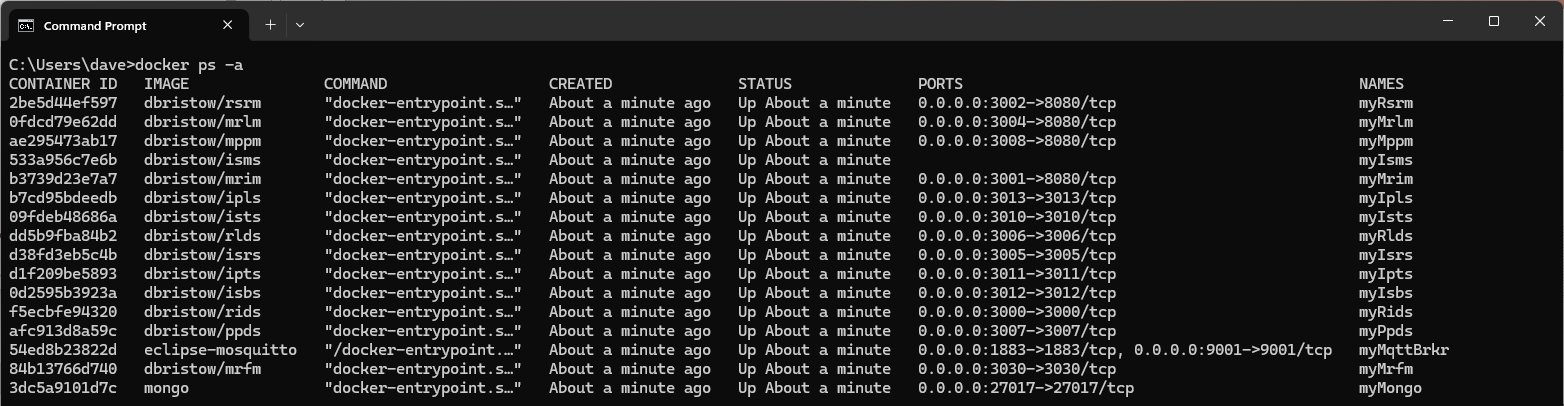
\includegraphics[scale=0.4]{win3.png}
    \caption{Windows Docker PS}
    \label{fig:docker-cmds-2}
\end{figure}
\begin{figure}[H]
    \centering
    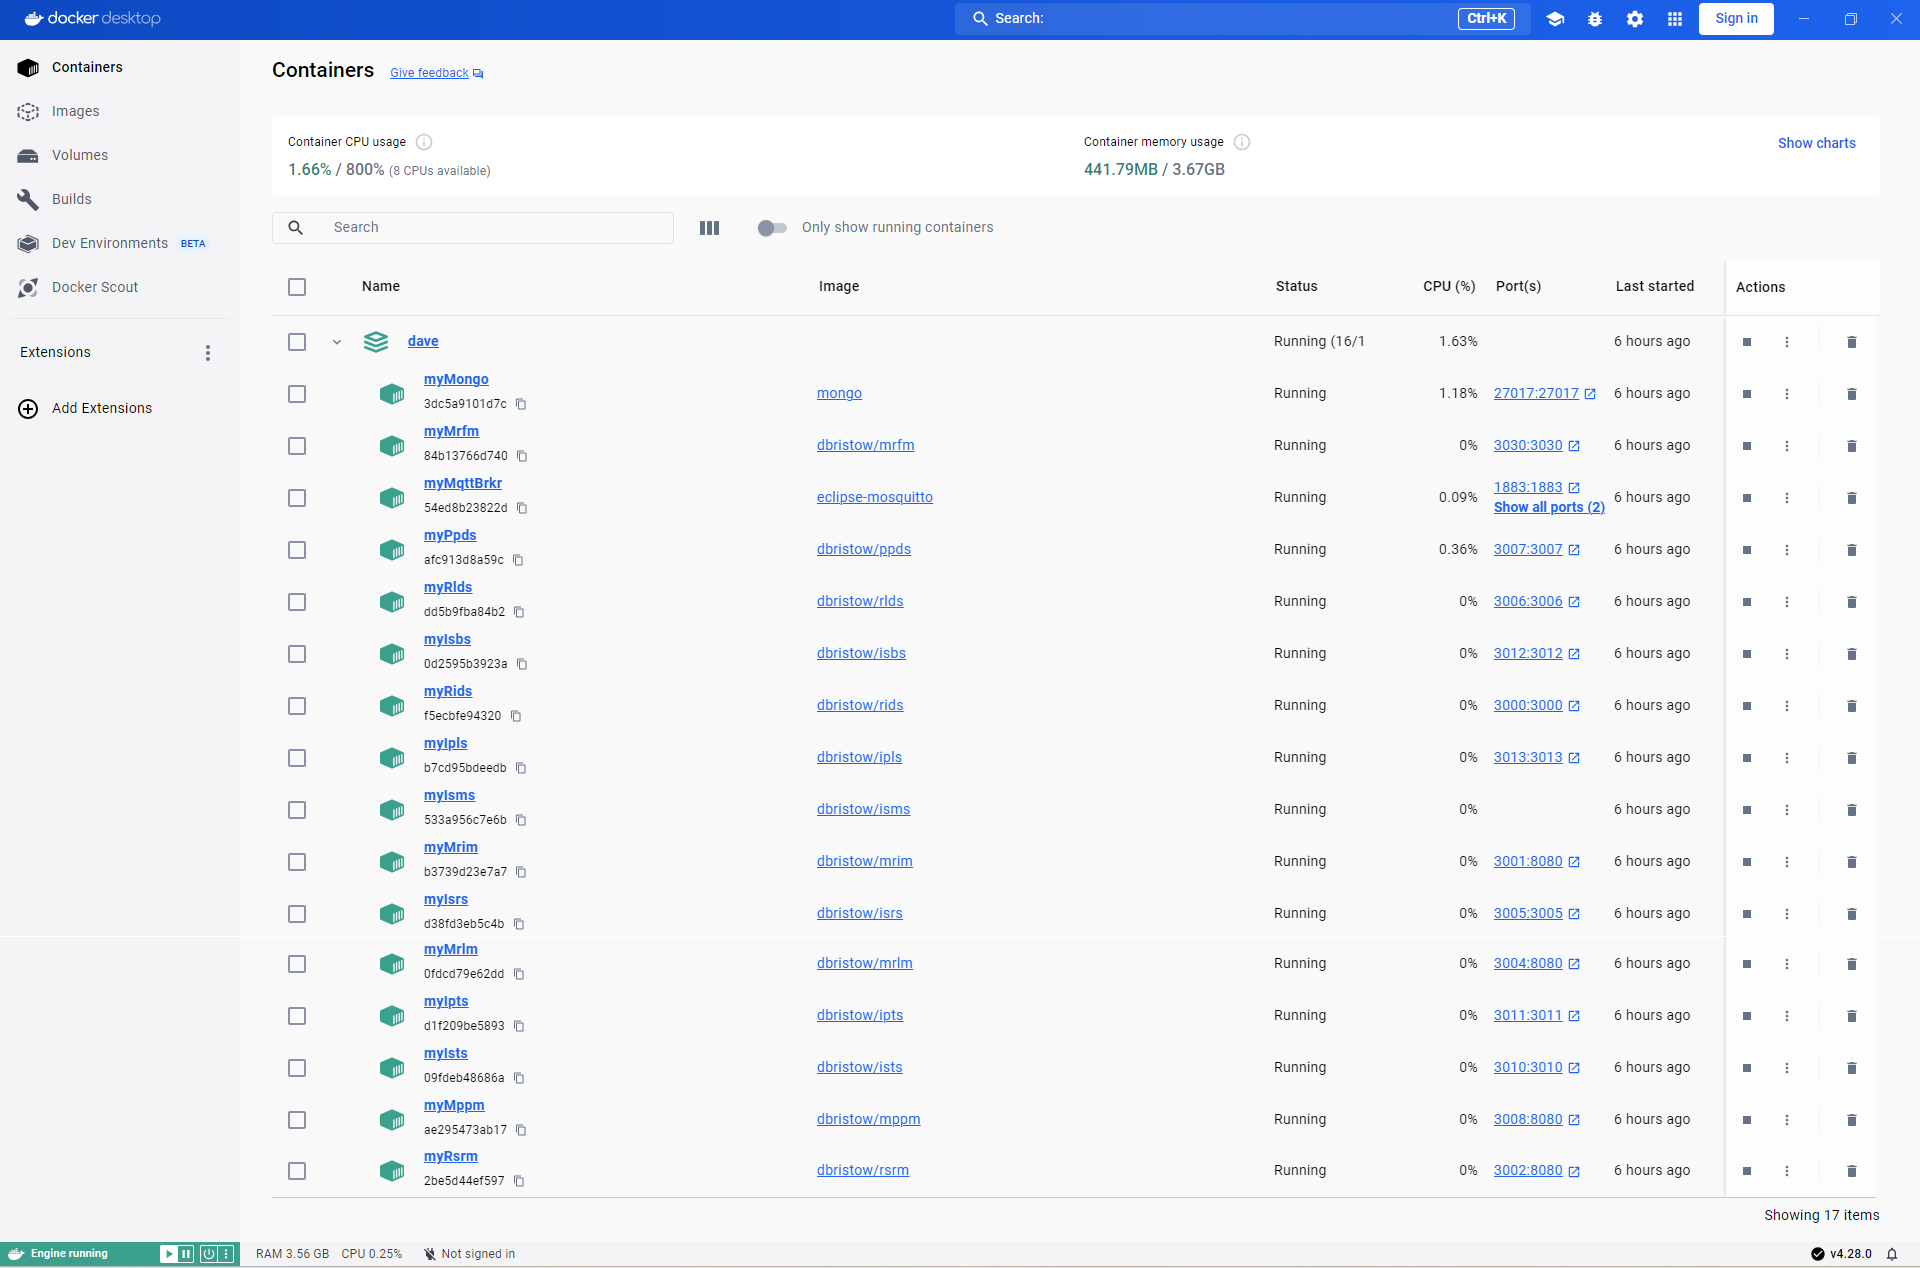
\includegraphics[scale=0.33]{dd-containers.png}
    \caption{Windows Docker Desktop Containers}
    \label{fig:docker-cmds-2}
\end{figure}
Once the Docker containers are running, the \gls{rails} \glspl{spa} can be accessed from a web browser (Chrome). The following screenshots show the \gls{rails} \glspl{spa} running in a web browser.
\begin{figure}[H]
    \centering
    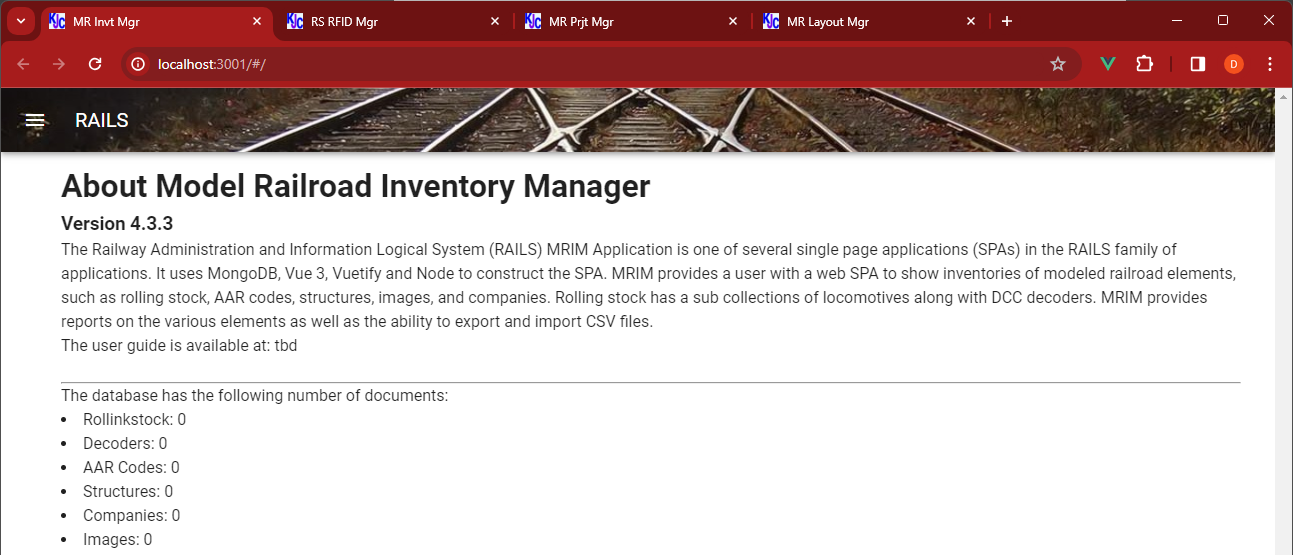
\includegraphics[scale=0.46]{mrim.png}
    \caption{RAILS MRIM Running}
    \label{fig:rails-mrim}
\end{figure}
\begin{figure}[H]
    \centering
    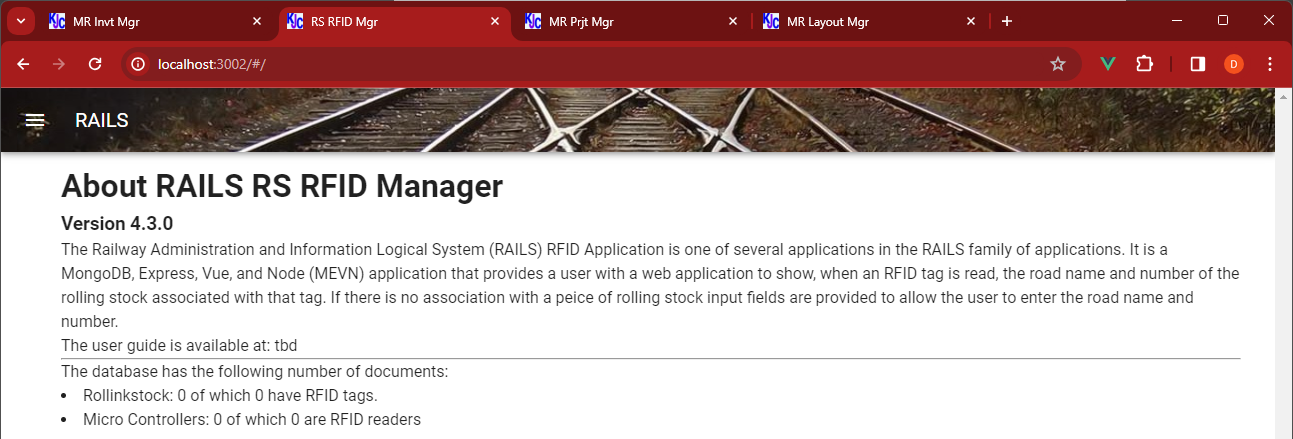
\includegraphics[scale=0.46]{rsrm.png}
    \caption{RAILS RSRM Running}
    \label{fig:rails-rsrm}
\end{figure}
\begin{figure}[H]
    \centering
    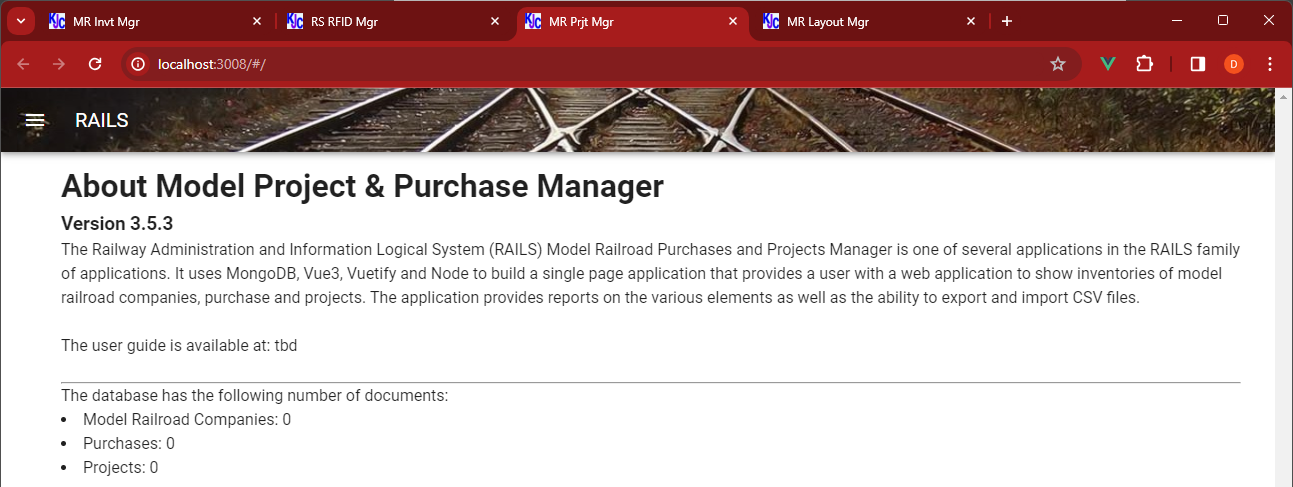
\includegraphics[scale=0.46]{mppm.png}
    \caption{RAILS MPPM Running}
    \label{fig:rails-mrim}
\end{figure}
\begin{figure}[H]
    \centering
    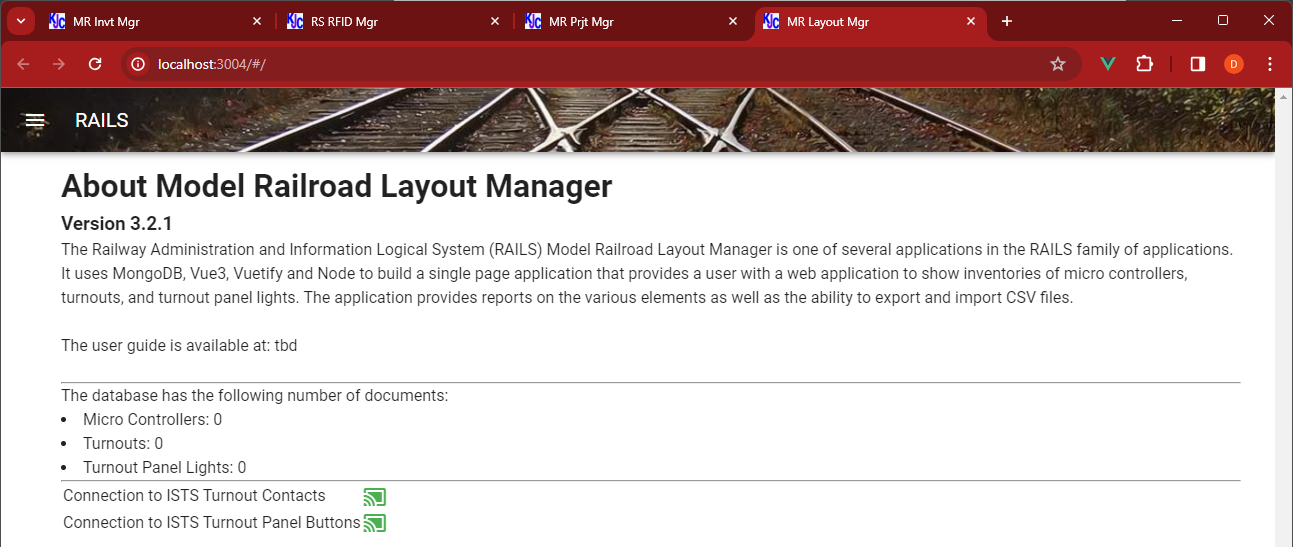
\includegraphics[scale=0.46]{mrlm.png}
    \caption{RAILS MRLM Running}
    \label{fig:rails-rsrm}
\end{figure}
The following screenshot shows the stoping and removal of the \gls{rails} Docker containers in a Windows environment.
\begin{figure}[H]
    \centering
    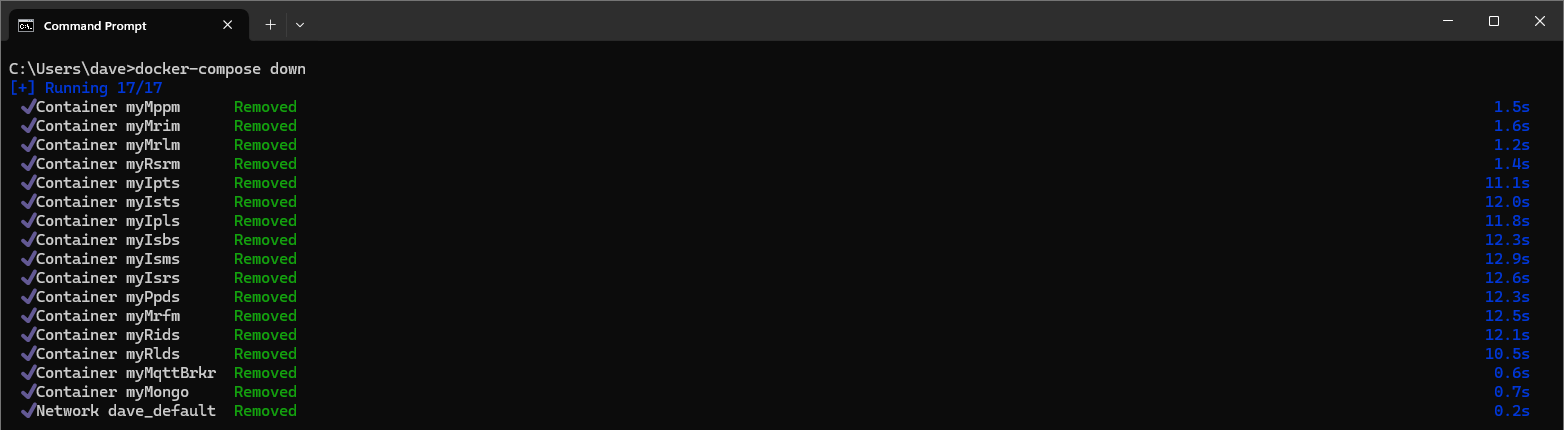
\includegraphics[scale=0.4]{win4.png}
    \caption{Windows Docker-Compose Down}
    \label{fig:docker-cmds-3}
\end{figure}
\newpage
\section{Docker in a Linux Environment}
\label{sec:linux-cmds}
The following screenshot shows the intial Docker commands used to create the Docker environment in a Linux environment. The yellow highlighted text represents the edits of the mosquitto configuration file using the vi editor.
\begin{figure}[H]
    \centering
    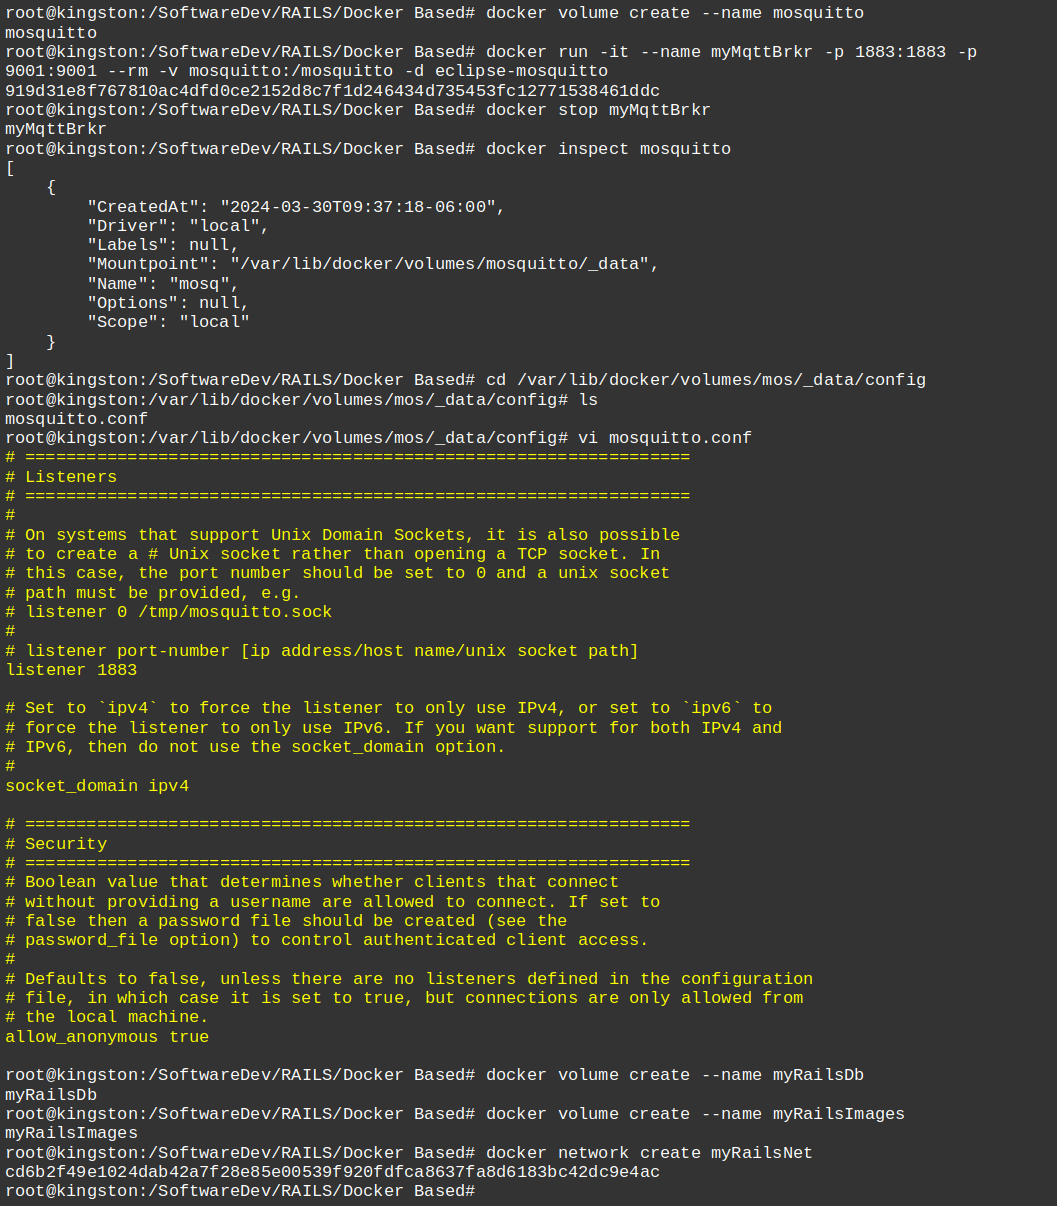
\includegraphics[scale=0.44]{win1l.png}
    \caption{Initial Linux Docker Commands}
    \label{fig:linux-docker-cmds}
\end{figure}
The following screenshots show the Docker command used to pull images and run the \gls{rails} Docker containers in a Linux environment. The pink elispes represent the multiple layers of the images being pulled from the Docker Hub.
\begin{figure}[H]
    \centering
    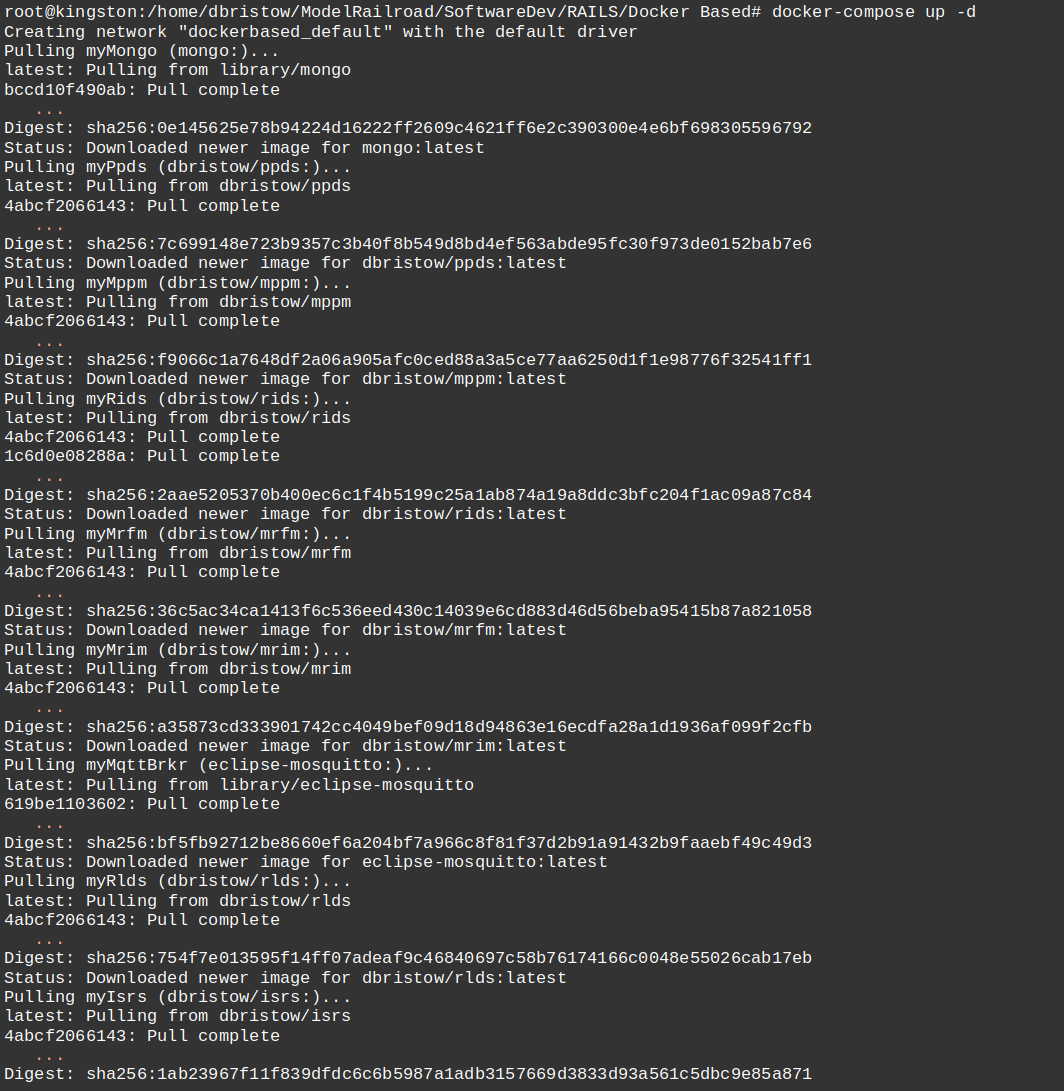
\includegraphics[scale=0.44]{win2l.png}
    \caption{Linux Docker-Compose Up}
    \label{fig:linux-docker-cmds-2}
\end{figure}
\begin{figure}[H]
    \centering
    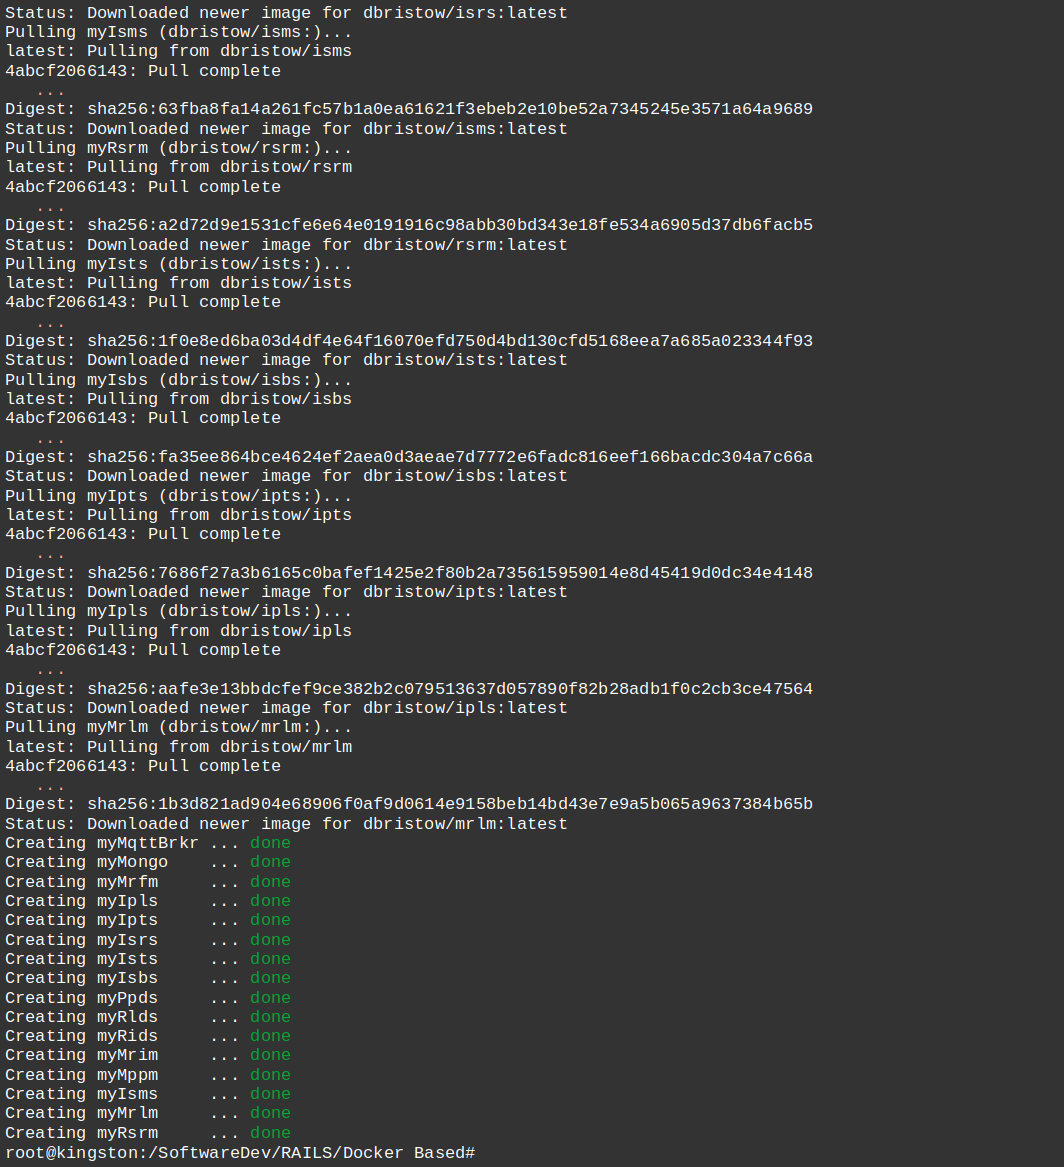
\includegraphics[scale=0.44]{win3l.png}
    \caption{Linux Docker-Compose Up Continued}
    \label{fig:linux-docker-cmds-3}
\end{figure}
The following screenshot shows a \gls{rails} \glspl{spa} running in a web browser (Chrome) in a Linux environment. The remaining \glspl{spa} can be accessed in the same manner.
\begin{figure}[H]
    \centering
    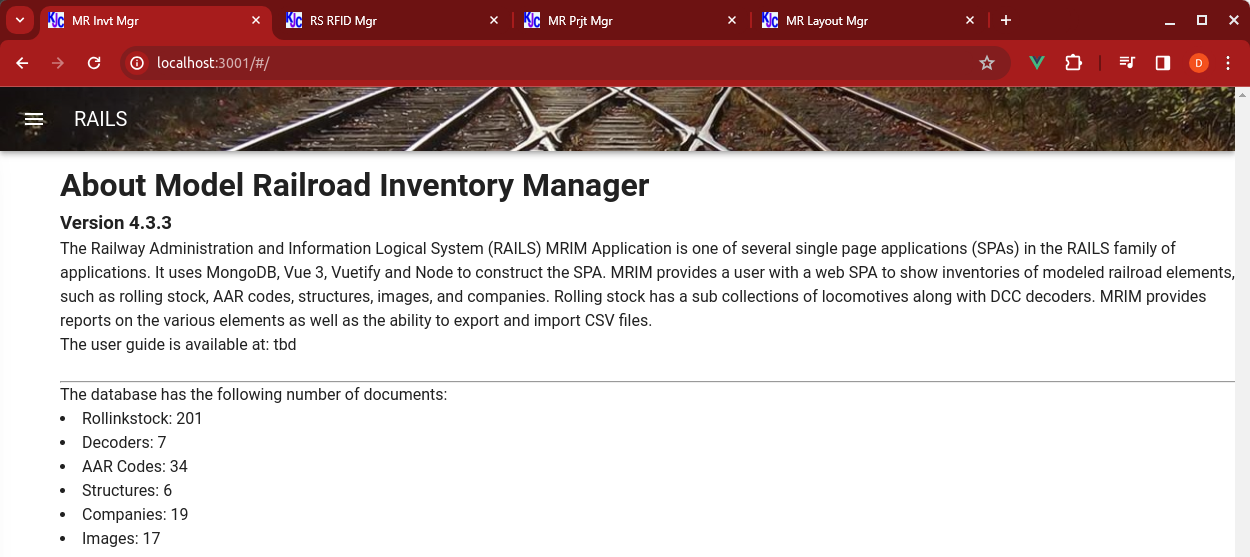
\includegraphics[scale=0.36]{mriml.png}
    \caption{RAILS MRIM Running}
    \label{fig:rails-mrim}
\end{figure}
The following screenshot shows the stoping and removal of the \gls{rails} Docker containers in a Linux environment.
\begin{figure}[H]
    \centering
    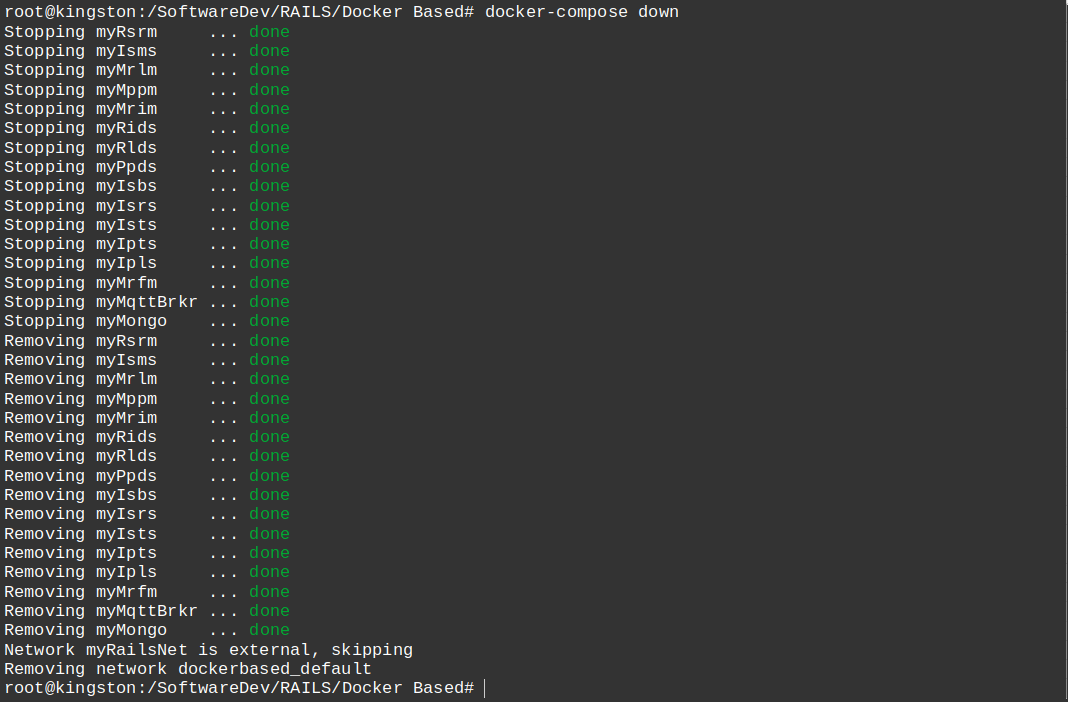
\includegraphics[scale=0.44]{win4l.png}
    \caption{Linux Docker-Compose Down}
    \label{fig:linux-docker-cmds-4}
\end{figure}
\section{Docker in a MacOS Environment}
\label{sec:mac-cmds}
Docker itself doesn't run directly on MacOS 14 (Mojave). This is because Docker relies on a Linux kernel for containerization, and MacOS uses a different kernel. 
Similar to Windows there is a Docker Desktop software package that provides a complete Docker experience on MacOS. It includes:
\begin{itemize}
\item Docker Desktop installs and runs a lightweight Linux \gls{vm} in the background. This  \gls{vm} typically uses LinuxKit, a minimal Linux distribution optimized for running Docker.
\item The Docker engine runs within the Linux \gls{vm}. This engine is responsible for managing Docker images, containers, and networks.
\item Docker Desktop provides a \gls{cli} for interacting with the Docker engine running in the VM. You can use familiar Docker commands to build, run, and manage containers.
\item Docker Desktop offers an optional GUI that allows you to manage containers visually.
\end{itemize}
The following screenshot shows the intial Docker commands used to create the Docker environment in a MacOS environment. Like Windows it is simpler to use Docker Desktop \gls{gui} to locate and edit the mosquitto configuration file.
\begin{figure}[H]
    \centering
    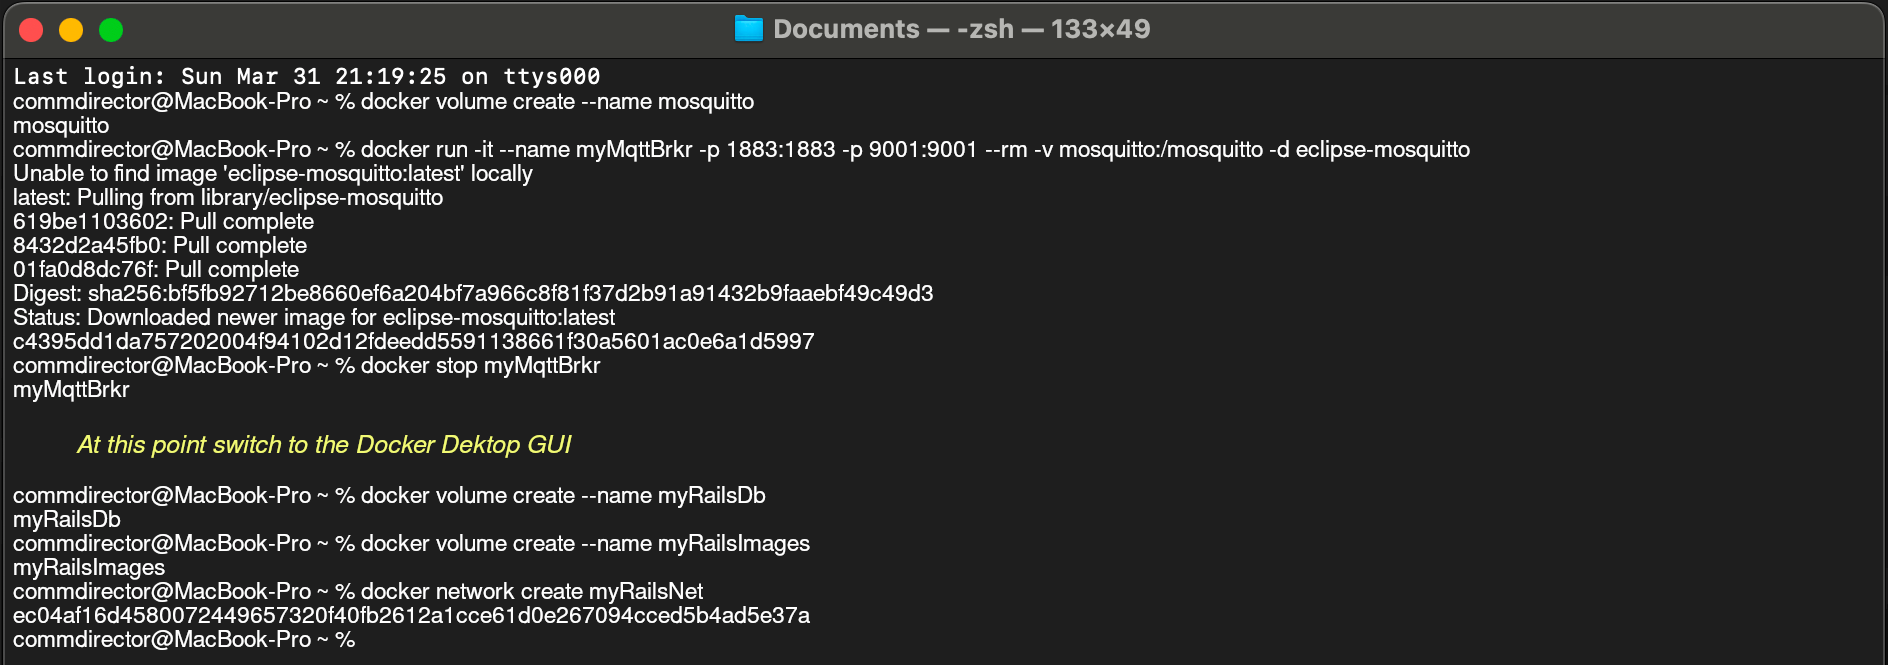
\includegraphics[scale=0.5]{win1m.png}
    \caption{Initial MacOS Docker Commands}
    \label{fig:mac-docker-cmds}
\end{figure}
The following screenshots show the Docker command used to pull images and run the \gls{rails} Docker containers in a MacOS environment.
\begin{figure}[H]
    \centering
    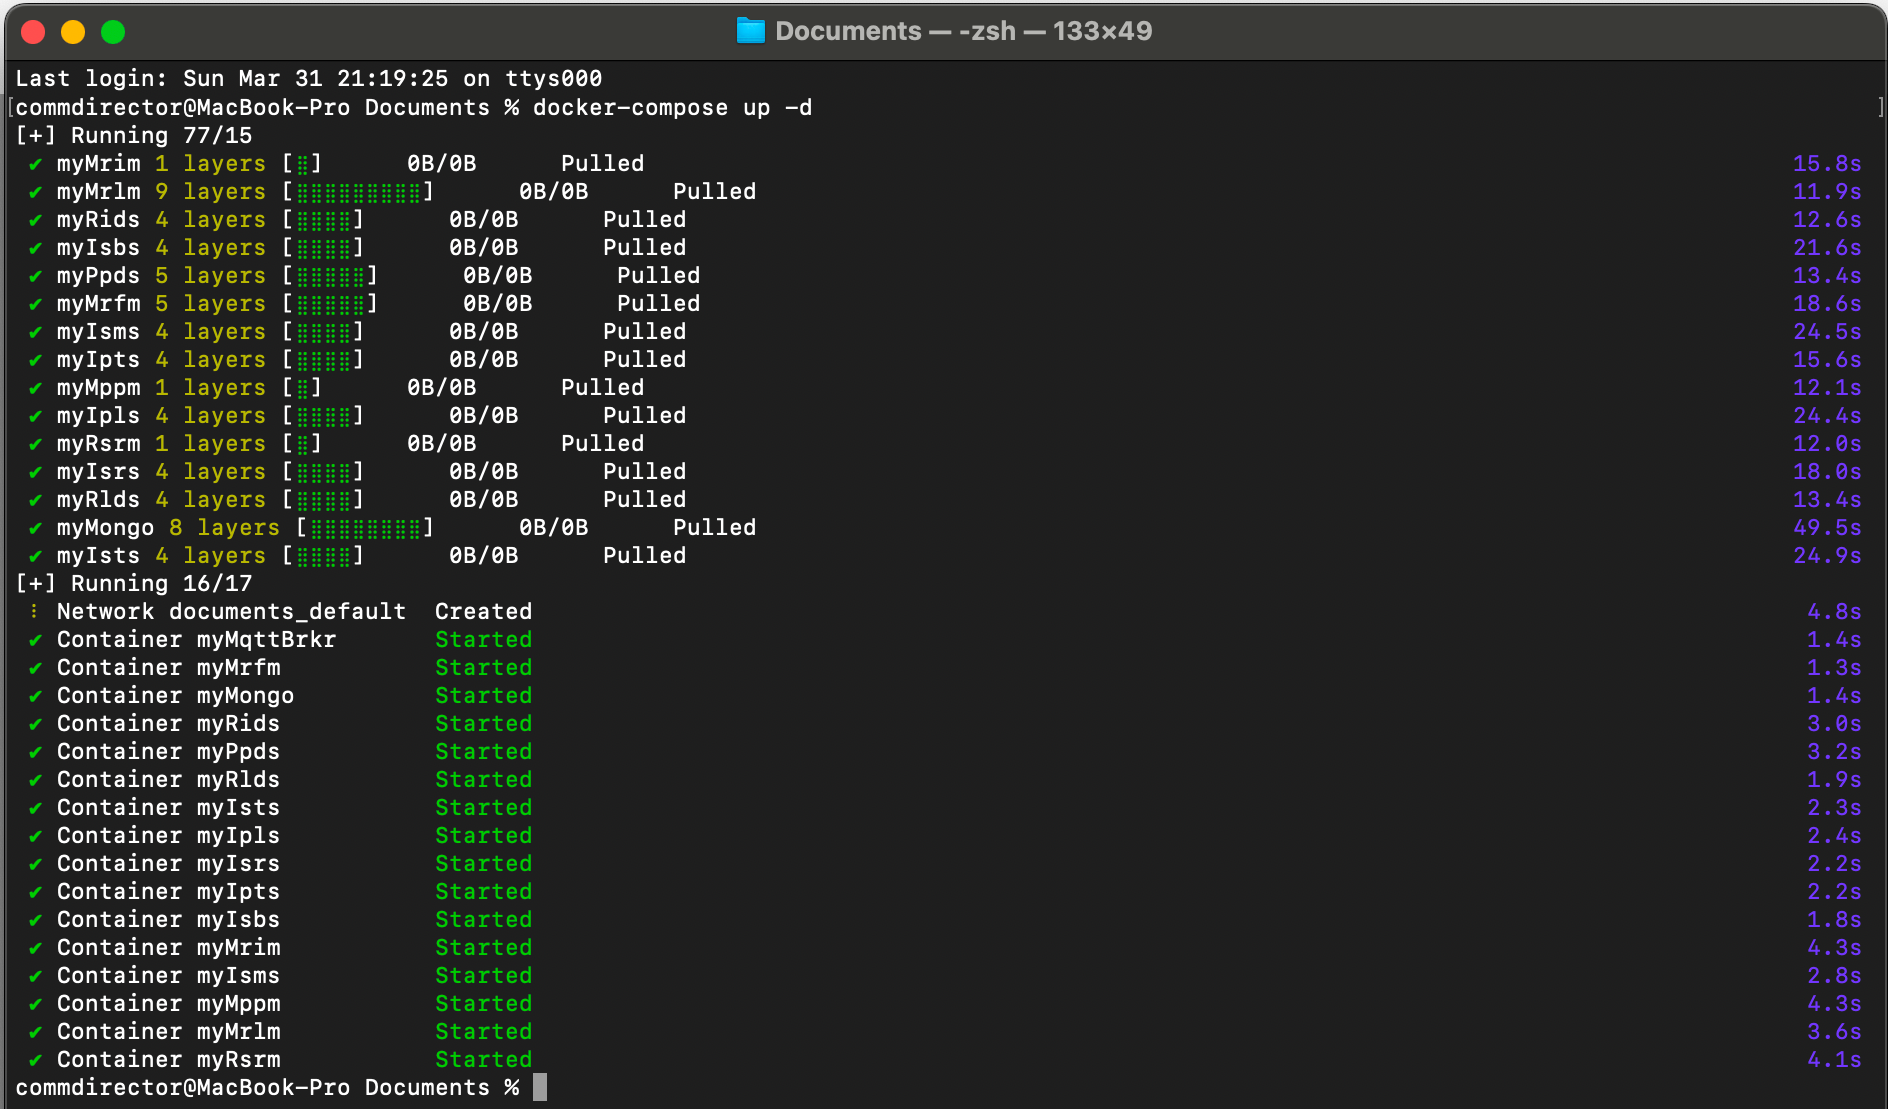
\includegraphics[scale=0.5]{win2m.png}
    \caption{MacOS Docker-Compose Up}
    \label{fig:mac-docker-cmds-2}
\end{figure}
The following screenshot shows a \gls{rails} \glspl{spa} running in a web browser (Safari) in a MacOS environment. The remaining \glspl{spa} can be accessed in the same manner.
\begin{figure}[H]
    \centering
    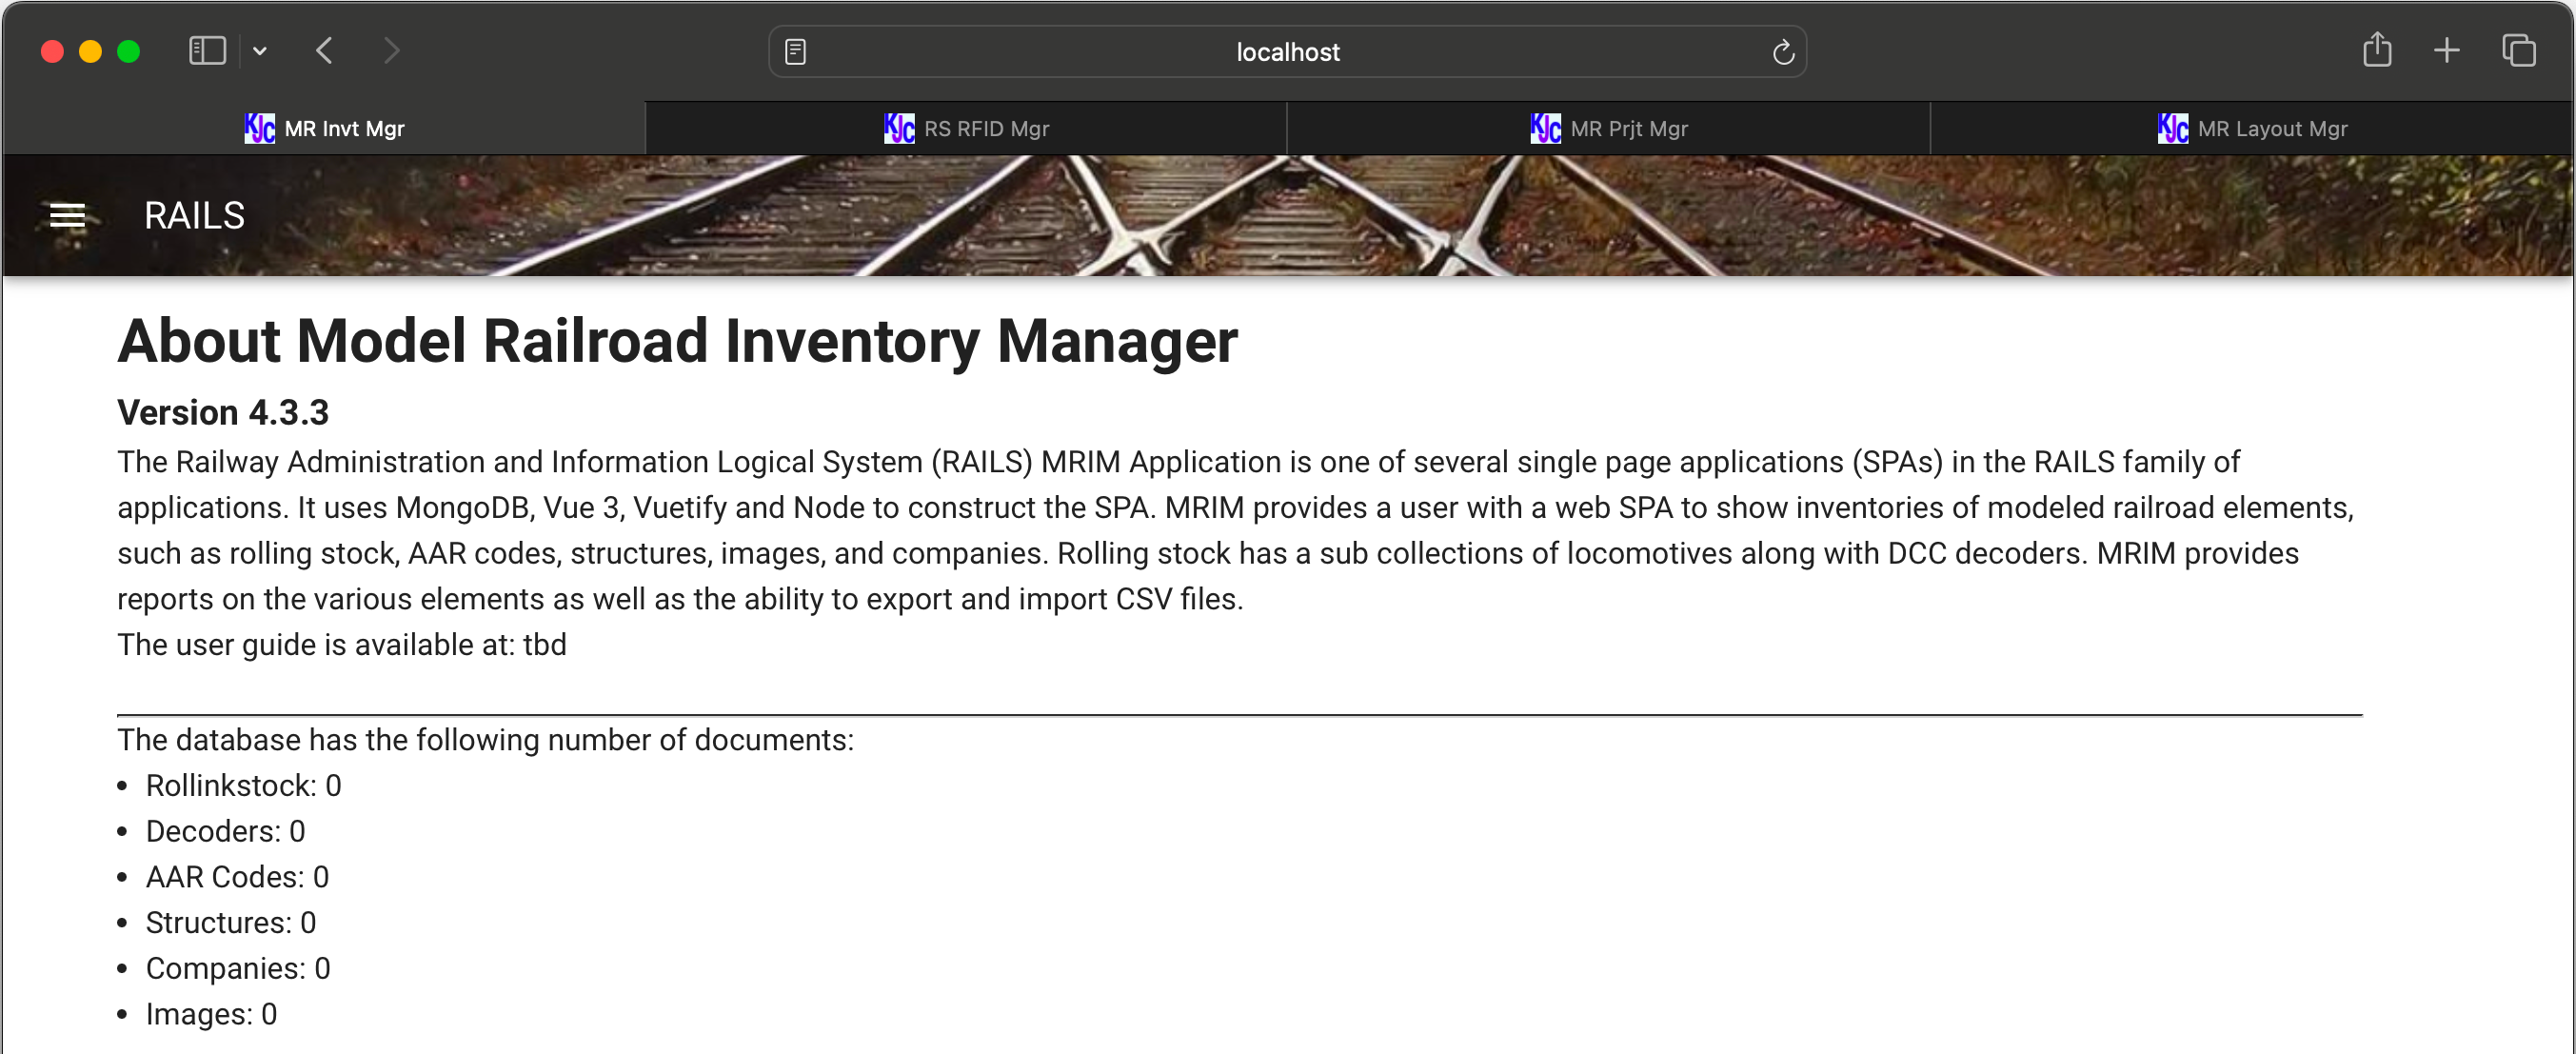
\includegraphics[scale=0.33]{mrimm.png}
    \caption{RAILS MRIM Running}
    \label{fig:rails-mrim}
\end{figure}
The following screenshot shows the stoping and removal of the \gls{rails} Docker containers in a Linux environment.
\begin{figure}[H]
    \centering
    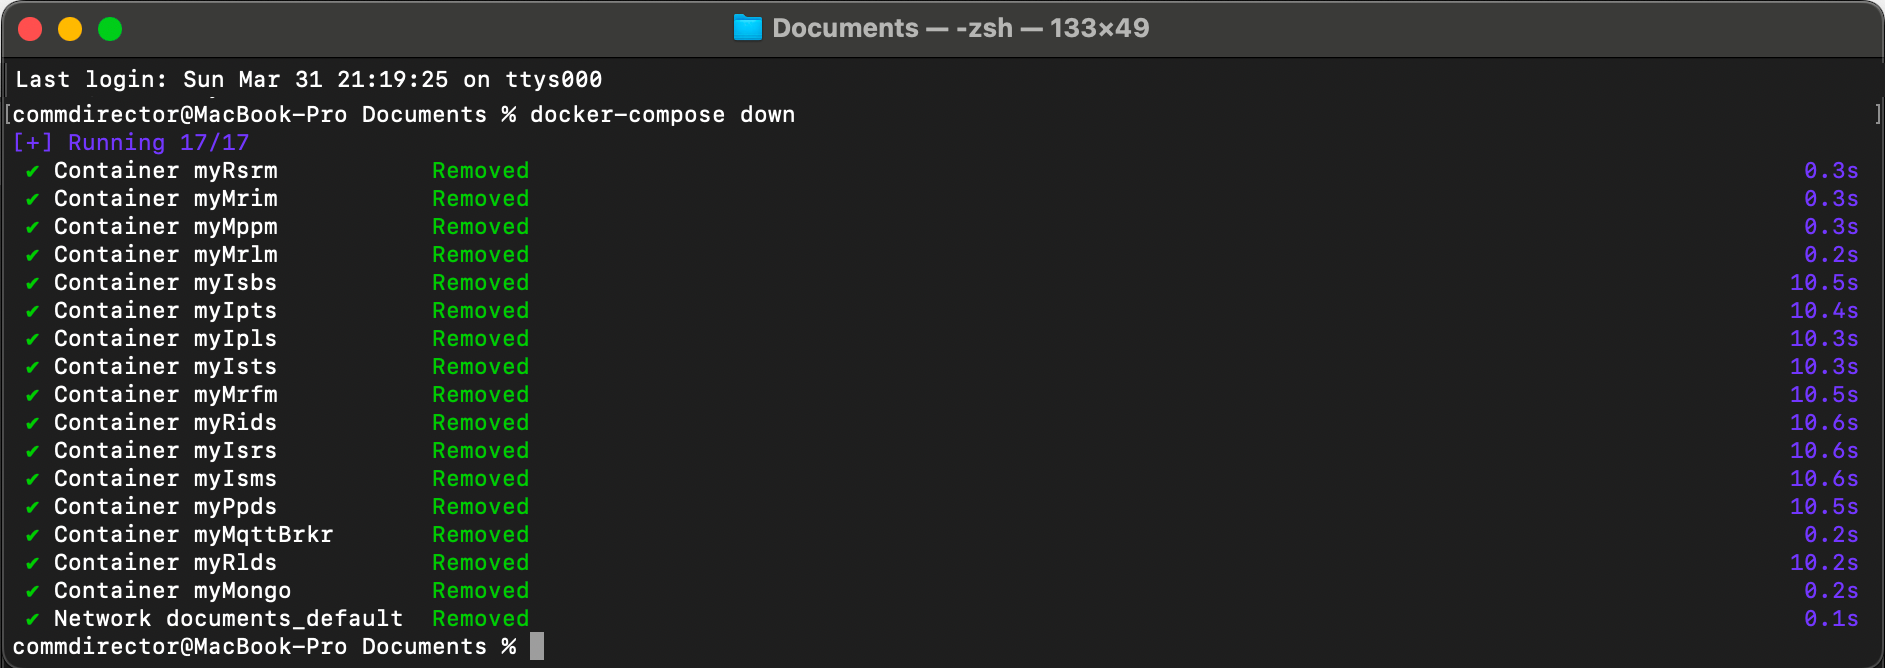
\includegraphics[scale=0.5]{win3m.png}
    \caption{MacOS Docker-Compose Down}
    \label{fig:mac-docker-cmds-3}
\end{figure}
\chapter{Docker Commands}
\label{app:dockercommands}
The following Docker commands may be useful when working with Docker images and containers related to the \ac{RAILS} \acp{SPA}.
\begin{itemize}
    \item \texttt{docker ps} - List running containers.
    \item \texttt{docker ps -a} - List all containers including those that have been stopped.
    \item \texttt{docker images} - List images.
    \item \texttt{docker run -d --name <container-name> <image-name>} - Run a container from an image.
    \item \texttt{docker stop <container-name>} - Stop a running container.
    \item \texttt{docker rm <container-name>} - Remove a container.
    \item \texttt{docker rmi <image-name>} - Remove an image.
    \item \texttt{docker inspect <container-name> | <volume-name> } - Display detailed information about a container or volume.
    \item \texttt{docker-compose up -d} - Start the services defined in the Docker Compose file.
    \item \texttt{docker-compose down} - Stop the services defined in the Docker Compose file.
\end{itemize}
%%========================================================================
\backmatter
\chapter{Acronyms}
\begin{acronym}
\acro{API}{Application Program Interface}
\acro{CLI}{command-line interface}
\acro{DCC}{Digital Command and Control}
\acro{DS}{Data Services}
\acro{EJB}{Enterprise Java Bean}
\acro{GUI}{Graphic User Interface}
\acro{IDE}{Integrated Development Environment}
\acro{I/O}{input/output}
\acro{IR}{Infrared}
\acro{IoT}{Internet of Things}
\acro{IPLS}{IoT Publisher Turnout Panel Light Services}
\acro{IPTS}{IoT Publisher Turnout Services}
\acro{ISBS}{IoT Subscriber Turnout Panel Button Services}
\acro{ISLS}{IoT Subscriber Location Services}
\acro{ISMS}{IoT Subscriber Micro-controller Services}
\acro{ISRS}{IoT Subscriber RFID Services}
\acro{ISTS}{IoT Subscriber Turnout Services}
\acro{JEE}{Java Enterprise Edition}
\acro{JSF}{JavaServer Faces}
\acro{MQTT}{Message Queuing Telemetry Transport}
\acro{MRFM}{Model Railroad File Manager}
\acro{MRIM}{Model Railroad Inventory Manager}
\acro{MPPM}{Model Projects and Purchase Manager}
\acro{MQTT}{Message Queuing Telemetry Transport}
\acro{MRLM}{Model Railroad Layout Manager}
\acro{QoS}{quality of service}
\acro{SPA}{Single Page Application}
\acro{PPDS}{Plans and Purchases Data Services}
\acro{RAILS}{Railway Administration and Information Logical System}
\acro{RDB}{Relational Database}
\acro{RIDS}{Railroad Inventory Data Services}
\acro{RLDS}{Railroad Layout Data Services}
\acro{RFID}{Radio Frequence Identification}
\acro{RSRM}{Rollingstock RFID Manager}
\acro{SOA}{Services Oriented Architecture}
\acro{UI}{User Interface}
\acro{VCS}{version control system}
\acro{VS Code}{Visual Studio Code}
\end{acronym}

\end{document}